\documentclass[11pt,a4paper]{ctexart}
\usepackage[margin=2.4cm]{geometry}
\usepackage{amsmath,amssymb,amsthm}
\usepackage{booktabs}
\usepackage{unicode-math}
\setmathfont{Latin Modern Math}[BoldFont={Latin Modern Math},BoldFeatures={FakeBold=1.5}]
\usepackage{graphicx}
\graphicspath{{../figures/}{../paper/figures/}}
\usepackage{enumitem}
\usepackage{natbib}
\usepackage{xurl}
\setlength{\emergencystretch}{2em}
\usepackage[colorlinks=true,linkcolor=black,citecolor=black,urlcolor=blue]{hyperref}

\newtheorem{theorem}{定理}
\newtheorem{lemma}{引理}
\newtheorem{proposition}{命题}
\newtheorem{corollary}{推论}
\theoremstyle{definition}
\newtheorem{remark}{注}
\renewcommand{\proofname}{证明}
\xeCJKDeclareCharClass{Default}{"2019}
\newcommand{\E}{\mathbb{E}}
\newcommand{\F}{\mathcal{F}}
\newcommand{\ind}{\mathbf{1}}
\newcommand{\Sw}{\mathcal{S}}
\DeclareMathOperator{\cov}{cov}
\DeclareMathOperator*{\plim}{plim}

\title{传播尺度的双重差分：反馈与空间传染下的序贯矩估计与诊断边界}
\author{}
\date{中文阅读稿。图 1--3 取自英文稿；表与网络附录的编号均指英文稿及其网络支持材料。}

\begin{document}
\maketitle

\begin{abstract}
\noindent
报告病例面板是评估非药物干预的标准数据，但结局尺度上的双重差分依赖三条疫情数据不满足的假设：传播自我激发，政策随发病上升而实施，单元之间相互感染。
本文把平行趋势放在带邻近输入感染压力的更新模型的对数再生数上，并用前向准差分广义矩估计（QD-GMM）估计政策效应；前向准差分消去不受限制的单元效应，仅由过去信息构造的工具变量允许基于发病率的政策反馈。
排除未建模的同周跨集群传播时，集群矩得分按周构成鞅差阵列，因此常规聚类稳健夹心方差无需空间校正即可适用，周效应有闭式剖面解。
内置诊断明确区分工作模型参数与结构因果效应：剖面传染方程揭示边界多根，得分形式过度识别检验（$J_{LM}$）对照校准零分布解读，剖面化 Stock--Wright 集合则绕开边界选根。
在包含反馈、溢出与过度离散的预设模拟（$R=8000$）中，直接效应偏倚介于 $-0.002$ 与 $0.001$ 之间（覆盖率 94.5\%--95.4\%），显著优于常用比较量，而边界与同周（$w_0=0.3$）实验界定了方法有效域。
在对德国 2015--2019 年 400 个县、16 个州水痘监测数据（$w_0<10^{-5}$）的事后压力测试中，工作模型给出负向政策层面对比（$\hat\tau+\hat\kappa=-0.239$，$t_{15}$ 区间 $-0.364$ 至 $-0.115$；WCR 得分 $-0.419$ 至 $-0.139$），两步对数 $R$ 回归则在 58.8\% 零计数下发生符号反转。但被拒绝的过度识别检验（$p_{\mathrm{cal}}=0.004$）、总尺度起始周即刻下降（$-0.208$）、短期假期先降后弹安慰剂、南部非轮换州以及区域季节控制敏感性共同表明，尚不能据此得出无混杂的因果减毒归因。
\end{abstract}

\noindent\textbf{关键词：} 因果推断；诊断边界；双重差分；广义矩估计；传染病流行病学；干扰；更新方程

\section{引言}
\label{s:intro}

按县或地区汇总的报告病例面板是评估停课、出行限制与社区防控等非药物干预的标准数据。实践中，干预效应常通过事件研究、病例增长或对数病例的双向固定效应回归、区域比较及合成控制来估计
\citep{hsiang2020anticontagion,chernozhukov2021masks,mitze2020masks}，这些方法都沿用了政策评估中的双重差分逻辑\citep{callaway2021did,roth2023trending,haber2021impact}。
然而疫情数据在三处同时动摇结局尺度的双重差分：周病例由更早数周病例经代际间隔生成\citep{wallinga2004different,fraser2007estimating,wallinga2007generation}，即使无政策，病例数或对数病例上的平行趋势也会失效\citep{gauthier2021twfe,feng2024parallel}；政策实施往往响应上升的发病率，处理依赖过去结局，常规单元固定效应失去依据\citep{imai2019fixed,zhang2025timevarying}；单元在空间上相互耦合，感染跨越边界且邻居政策改变接触模式\citep{hudgens2008interference,halloran2016dependent,aronow2017exposure}，忽略溢出将扭曲估计\citep{enriquez2025spillovers}。

现有方法各自只解决了其中一部分。\citet{feng2024parallel} 把平行趋势放在基于队列的对数有效再生数上，未纳入溢出，且依赖第一步再生数估计，后者受小计数 Jensen 偏倚与代际间隔失真影响\citep{gostic2020practical}。
贝叶斯形式\citep{flaxman2020npi,brauner2021npi,bhatt2023semimech}或频率学形式\citep{bong2024frequentist,bong2024augmented}的半机理更新模型、SIR 启发的无混杂性\citep{callaway2023pandemic}及结构增长模型\citep{chernozhukov2021masks}均以观测历史为条件，未消去不受限制的单元效应。
时空计数模型\citep{held2005hhh,meyer2014powerlaw,alaimo2024poissonar}刻画空间耦合，却未处理反馈实施。
空间与网络双重差分设计\citep{kosfeld2021spatial,butts2021spatial,forastiere2021network,xu2023did,sun2025didnetwork}在结局尺度上处理区域溢出，不含更新动力学与反馈。
前定回归元下的准差分序贯矩可消去乘性单元效应\citep{chamberlain1992sequential,wooldridge1997multiplicative,windmeijer2000moment,blundell2002count}，但尚未与更新传播、空间传染及形式化诊断整合。

本文将前向准差分广义矩（QD-GMM）置于传播尺度上，并配备显式的识别与失效模式诊断。本文不预设周度监测面板在所有场景下都能复原结构因果效应，而是精确界定参数何时点识别、何时会因诊断告警而降格为被拒绝工作模型的伪真值。
具体而言，我们把平行趋势放在带邻近输入感染压力的更新模型对数再生数上；前向准差分消去不受限制的单元效应；完全由观测过去构造的工具变量允许发病驱动反馈；政策溢出经由受处理邻居比例进入模型。
由此得到三项方法学结果。第一，在排除未建模同周跨集群传播的条件下，尽管存在滞后集群间传染，矩贡献按周构成鞅差阵列，常规聚类稳健夹心方差无需空间 HAC 校正即可适用，且周效应有闭式剖面解。
第二，在包含反馈、溢出、过度离散与小计数的预设模拟（$R=8000$）中，QD-GMM 复原直接效应的偏倚为 $-0.002$ 至 $0.001$，95\% 区间覆盖率为 94.5\% 至 95.4\%，而结局尺度、泊松固定效应与两步对数 $R$ 比较量均系统性失效；匹配的边界（$\phi_0=0$）与同周传播（$w_0=0.3$）实验进一步界定了方法有效域。
第三，内置诊断——揭示多根的剖面传染方程、对照有限样本校准零分布解读的过度识别检验（$J$ 或满秩得分形式 $J_{LM}$）、Stock--Wright 识别稳健集、总政策尺度事件时间剖面与报告率敏感性检验——直接从观测数据中检出设定与监测失效。

我们在德国 400 个县、16 个联邦州 2015--2019 年的周度水痘（\emph{Windpocken}）监测面板（115,129 例）上对上述框架进行压力测试\citep{cauchemez2008school,jackson2014varicella,adda2016economic,vonbismarckosten2022schools,isphording2021schools}。
水痘 14 天平均代际间隔\citep{vink2014serial}使同周传播份额低至 $w_0=2.6\times 10^{-6}$，而稀疏县周计数（零计数 58.8\%）对定理~\ref{thm:bias} 提供了直接检验。
实际监测数据中，两步 EpiEstim 对数 $R$ 回归在县级反号为 $+0.064$，而在 NUTS-2 聚合（零计数 2.9\%）后反转为 $-0.102$；$\log(Y+1)$ 双向固定效应衰减至 $-0.102$。
基准 QD-GMM 工作模型给出负向政策层面对比（$\hat\tau+\hat\kappa=-0.239$，95\% $t_{15}$ 区间 $-0.364$ 至 $-0.115$；限制得分野 bootstrap $-0.419$ 至 $-0.139$）及内部耦合根 $\hat\phi=0.326$。
但框架内诊断阻止了将该数字解释为无混杂的 21.3\% 因果减毒效应：$J_{LM,\mathrm{oi}}$ 拒绝滞后工作模型矩条件（校准 $p=0.004$），总政策尺度事件时间估计在暑假起始周即出现 $-0.208$ 下降（$p=0.049$），短期非暑期假期均呈先降后弹（滞后 2 正向回补），南部巴符州与巴伐利亚州从不轮换起始周且剔除该两州或控制四大区 $\times$ 周效应后置信区间均包含零。
第~\ref{s:methods}--\ref{s:discussion} 节依次阐述理论、模拟、德国压力测试与适用范围；网络附录 A--F 给出证明、改写的比较量结果、数值核对、补充模拟、数据来源、少簇校准与完整诊断。

\section{方法}
\label{s:methods}

\subsection{设定、潜在结局与估计目标}

单元 $i=1,\dots,N$（县）划分为 $G$ 个集群（州），$g(i)$ 表示单元 $i$ 所在集群，集群规模 $n_g$ 有界。
周记为 $t=1-S,\dots,T$，其中周 $1,\dots,T$ 是估计窗口，此前 $S$ 周只用于构造滞后。$Y_{it}$ 为报告的新增病例，$D_{it}\in\{0,1\}$ 为政策，$t\le 0$ 时 $D_{it}=0$。
若单元在第 1 周之前已暴露，下文的潜在结局与期望均以 $(Y_{\le 0},D_{\le 0})$ 为条件，$\mathbf 0$ 表示自第 $1$ 周起撤除政策。
$W=(W_{ij})$ 是已知、非负、行归一化且对角为零的空间权重矩阵，$\bar D_{it}=\sum_j W_{ij}D_{jt}$ 为处于政策下的邻居比例。
给定已知的周代际间隔权重 $w_1,\dots,w_S\ge 0$，$\sum_s w_s=1$\citep{wallinga2007generation}，本地、输入与总感染压力分别记为 $L_{it}=\sum_{s=1}^{S} w_s Y_{i,t-s}$、$N_{it}=\sum_{s=1}^{S} w_s \sum_{j} W_{ij}Y_{j,t-s}$ 与 $\Lambda_{it}(\phi)=L_{it}+\phi N_{it}+\omega_i$，其中 $\omega_i>0$ 为很小的已知背景输入项。
取 $\theta=(\gamma_2,\dots,\gamma_T,\tau,\kappa,\phi)$，$\gamma_1=0$，均值函数定义如下：
\begin{equation}
m_{it}(\theta)=\exp(\gamma_t+\tau D_{it}+\kappa\bar D_{it})\,\Lambda_{it}(\phi).
\label{eq:mean}
\end{equation}

潜在结局 $Y_{it}(\mathbf d)$ 以整个政策路径 $\mathbf d=(\mathbf d_1,\dots,\mathbf d_T)$、$\mathbf d_t\in\{0,1\}^N$ 为索引，从而允许单元间的干扰\citep{hudgens2008interference}。
$H_{t-1}(\mathbf d)$ 为截至第 $t-1$ 周所有单元结局的潜在历史，$\Lambda_{it}(\mathbf d;\phi)$ 由它算出。单元效应 $\alpha=(\alpha_1,\dots,\alpha_N)$ 不可观测。所用的信息流如下：
\[
\F_t=\sigma\bigl(\alpha,\ Y_{js}\ (j\le N,\ s\le t),\ D_{js}\ (j\le N,\ s\le t+1)\bigr).
\]
它包含在第 $t$ 周末决定、用于第 $t+1$ 周的政策。工具变量是 $\F_{t-1}$ 可观测部分的函数。

目标参数由下文假设 A1 的传播模型定义。\emph{直接传播效应} $\tau$ 是单元条件再生数
$R_{it}(\mathbf d)=\E\{Y_{it}(\mathbf d)\mid\alpha,H_{t-1}(\mathbf d)\}/\Lambda_{it}(\mathbf d;\phi_0)$
在本单元有无政策两种情形下的对数比，历史与邻居政策保持不变。\emph{政策溢出} $\kappa$ 是处于政策下的邻居比例的相应效应，\emph{传染耦合} $\phi$ 是邻居近期病例的相对传染力。
对实施后单元周的集合 $\mathcal P$，\emph{避免病例数}定义如下：
\begin{equation}
\psi_{\mathcal P}=\E\sum_{(i,t)\in\mathcal P}\{Y_{it}(\mathbf 0)-Y_{it}\},
\label{eq:psi}
\end{equation}
其中 $\mathbf 0$ 为处处无政策的路径；$\psi_{\mathcal P}$ 包含经更新过程和跨单元的传播。

\subsection{假设}

\begin{description}[leftmargin=3.6em]
\item[A1（带平行对数传播趋势的更新模型）] 对任意政策路径 $\mathbf d$、单元 $i$ 与周 $t\ge1$，\\
$\E\{Y_{it}(\mathbf d)\mid \alpha,H_{t-1}(\mathbf d)\}=\exp(\alpha_i+\gamma_{t}+\tau_0 d_{it}+\kappa_0\bar d_{it})\Lambda_{it}(\mathbf d;\phi_0)$。
\item[A2（无预期与序贯可忽略）] (a) $Y_{it}(\mathbf d)$ 只通过 $\mathbf d_1,\dots,\mathbf d_t$ 依赖 $\mathbf d$。
(b) 对每个 $t$ 及满足 $\Pr(D_{1:t}=\mathbf d_{1:t})>0$ 的 $\mathbf d$，
$\E\{Y_{it}(\mathbf d)\mid\alpha,H_{t-1}(\mathbf d),D_{1:t}=\mathbf d_{1:t}\}=\E\{Y_{it}(\mathbf d)\mid\alpha,H_{t-1}(\mathbf d)\}$。
\item[A3（一致性）] $Y_{it}=Y_{it}(D)$。
\item[A4（集群间条件独立）] 对每个 $t$，给定 $\F_{t-1}$，集群向量 $(Y_{it})_{i:g(i)=g}$，$g=1,\dots,G$，相互独立。
这排除了同一周内跨越集群边界的感染（网络附录 A.12）。在网络附录 A（A.1 节）所述的有界度局部依赖结构 A4$'$ 下，A4 成立并蕴含大数定律 (L)。
\item[A5（压力为正）] 对所有 $i$、$t$ 与 $\phi\in[0,\bar\Phi]$，$\Lambda_{it}(\phi)\ge c>0$。$\bar\Phi$ 是 $\phi$ 参数空间的上界，区别于第~\ref{ss:estimation} 节定义的工具参考值 $\bar\phi$。
\item[A6（正则性）] 见网络附录 A.1：参数空间紧且 $\theta_0$ 为内点；矩的控制条件；下文定义的极限 $\bar g$、$\Gamma$、$\Omega$ 存在且 $\Omega$ 正定；$\bar g(\theta)=0$ 仅在 $\theta_0$ 处成立；$\Gamma$ 满秩。
\item[A7（报告）] 报告病例为 $Y_{it}=c_ic_tI_{it}$，其中 $I_{it}$ 为感染数，$c_i>0$ 为单元报告因子，$c_t>0$ 为周报告因子。
\end{description}

A1 要求未处理路径在对数尺度上平行（$\log R_{it}(\mathbf 0)=\alpha_i+\gamma_t$），同时允许与实施相关的任意单元水平 $\alpha_i$，以及不受限制的过度离散和聚集。
A2(b) 是均值形式的序贯随机化\citep{robins2000msm,blackwell2018make}，允许政策依赖 $\alpha$ 与完整的过去历史 $\F_{t-1}$（反馈），但不依赖同期冲击；邻居政策通过 $\kappa$ 进入，因此各州各自应对所产生的协调效应\citep{holtz2020interdependence}属于估计目标的一部分。
A4 允许集群内相关和滞后的跨集群传染，只排除未建模的同周跨集群冲击；当各州对全国总量作出反应时 A4$'$ 不成立，(L) 由此成为高层条件。只要 $\omega_i\ge c$，A5 即成立。

\begin{proposition}[报告率]
\label{prop:ascertainment}
设 A1 对感染数成立，感染压力为 $\Lambda^{I}_{it}$，报告病例满足 A7。再设报告压力使用背景项 $\omega^{Y}_{it}=c_ic_{t-1}\omega^{I}_i$，且 $\phi_0=0$ 或在 $W_{ij}>0$ 时总有 $c_i=c_j$。
(a) 若 $s=1,\dots,S$ 时 $c_{t-s}=c_{t-1}$，则报告病例满足 A1，$\alpha_i$、$\tau_0$、$\kappa_0$、$\phi_0$ 不变，$\gamma_t$ 换为 $\gamma_t+\log(c_t/c_{t-1})$。
(b) 否则 $|\log\Lambda^{Y}_{it}-\log(c_ic_{t-1}\Lambda^{I}_{it})|\le\max_{1\le s\le S}|\log(c_{t-s}/c_{t-1})|$，第 $t$ 周对数再生数的误差不超过代际窗口内报告率的最大相对变化。
\end{proposition}

命题~\ref{prop:ascertainment} 假定报告是确定性的且没有延迟；在二项稀疏化下 A1 只近似成立，当 $\omega_i\ll L_{it}$ 时，固定的 $\omega_i$ 近似满足 $\omega^Y_{it}$ 所需的缩放。
在连通的县级邻接图上，所有邻居满足 $c_i=c_j$ 意味着全国统一的单元报告因子，因此 $\phi_0>0$ 时该命题涵盖监测率的时间趋势，不涵盖县间报告率差异，也不涵盖随政策改变的报告；后者的临界点见第~\ref{s:application} 节。

\subsection{准差分矩}
\label{ss:moments}

对 $t=1,\dots,T-1$，令 $r_{it}(\theta)=m_{it}(\theta)/m_{i,t+1}(\theta)$。前向准差分\citep{chamberlain1992sequential,wooldridge1997multiplicative}定义如下：
\begin{equation}
u_{it}(\theta)=Y_{i,t+1}\,r_{it}(\theta)-Y_{it}.
\label{eq:qd}
\end{equation}

\begin{lemma}[观测数据模型与矩]
\label{lem:moment}
在 A1--A3 下，对 $t\ge 1$ 有 $\E(Y_{it}\mid\F_{t-1})=\mu_{it}:=e^{\alpha_i}m_{it}(\theta_0)$；若 $\E|Y_{i,t+1}r_{it}(\theta_0)|<\infty$，则准差分 \eqref{eq:qd} 对 $t=1,\dots,T-1$ 满足 $\E\{u_{it}(\theta_0)\mid\F_{t-1}\}=0$。
\end{lemma}

由于 $r_{it}$ 是均值之比，单元效应 $e^{\alpha_i}$ 相消。面向序贯外生回归元乘性面板的前向准差分源自\citet{wooldridge1997multiplicative} 与\citet{windmeijer2000moment}；本文把它嵌入带空间传染与政策干扰的更新均值。
设 $z_{it}$ 为 $q$ 维、$\F_{t-1}$ 可测的工具变量。集群贡献与样本矩如下：
\[
g_g(\theta)=\sum_{i:g(i)=g}\sum_{t=1}^{T-1} z_{it}u_{it}(\theta),\qquad
\hat g(\theta)=G^{-1}\sum_{g=1}^{G}g_g(\theta).
\]
记 $\varepsilon_{is}=Y_{is}-\mu_{is}$，$r_{is}=r_{is}(\theta_0)$。

\begin{lemma}[鞅表示]
\label{lem:mds}
在 A1--A3 下，$g_g(\theta_0)=\sum_{s=1}^{T}\xi_{gs}$，其中 $\xi_{gs}=\sum_{i:g(i)=g}a_{is}\varepsilon_{is}$，权重如下，且为 $\F_{s-1}$ 可测：
\[
a_{is}=z_{i,s-1}r_{i,s-1}\ind(s\ge 2)-z_{is}\ind(s\le T-1).
\]
于是 $\E(\xi_{gs}\mid\F_{s-1})=0$，且
\[
\E(g_g{g_g}^{\top})=\sum_{s}\E(\xi_{gs}{\xi_{gs}}^{\top}).
\]
若 A4 也成立，则对 $g\ne h$ 有 $\E\{g_g(\theta_0)g_h(\theta_0)^{\top}\}=0$。
\end{lemma}

滞后传染使相邻集群的原始结局相关（网络附录 B），但在 A4 下集群得分向量仍不相关，因此聚类稳健方差无需空间 HAC 校正即可成立。

\subsection{识别}
\label{ss:ident}

令 $x_{it}(\phi)=(D_{it},\bar D_{it},N_{it}/\Lambda_{it}(\phi))^{\top}$，$e_t$ 为长度 $T-1$ 的第 $t$ 个单位向量；把周效应参数化为 $\delta_t=\gamma_{t+1}-\gamma_t$，于是 $\theta=(\delta^{\top},\beta^{\top})^{\top}$，$\beta=(\tau,\kappa,\phi)^{\top}$，$p=T+2$。准差分的导数如下：
\begin{equation}
\frac{\partial u_{it}(\theta)}{\partial\theta^{\top}}=Y_{i,t+1}r_{it}(\theta)\bigl\{-{e_t}^{\top},\,x_{it}(\phi)^{\top}-x_{i,t+1}(\phi)^{\top}\bigr\}.
\label{eq:jac}
\end{equation}
此后 $\lim$ 均指 $G\to\infty$ 时的极限。令 $\bar g(\theta)=\lim G^{-1}\sum_g\E g_g(\theta)$，$\Gamma=\partial\bar g(\theta_0)/\partial\theta^{\top}$。在吸收式实施下，记切换者为 $\Sw_{i,t+1}=\ind(D_{it}=0,D_{i,t+1}=1)$。

\begin{theorem}[识别]
\label{thm:ident}
假设 A1--A3、A5 与 A6。
(a) $\bar g(\theta_0)=0$，雅可比矩阵由下式给出：
\[
\Gamma=\lim G^{-1}\sum_g\E\sum_{i\in g}\sum_{t}z_{it}\mu_{it}\{-{e_t}^{\top},x_{it}^{\top}-x_{i,t+1}^{\top}\}.
\]
若 $\operatorname{rank}\Gamma=p$，则 $\theta_0$ 是 $\bar g$ 在 $\theta_0$ 某邻域内的唯一零点；若在 $\theta_0$ 的某邻域内恒有 $\operatorname{rank}\partial\bar g(\theta)/\partial\theta^{\top}=r<p$，则 $\theta_0$ 局部不可识别。
(b) 设实施为吸收式，固定 $(\kappa,\phi)=(\kappa_0,\phi_0)$，使用工具 $s_{it}e_t$ 与 $s_{it}D_{it}$（$s_{it}>0$ 且 $\F_{t-1}$ 可测），并由周矩解出 $\delta$。
令 $A_t=\lim G^{-1}\E\sum_i s_{it}D_{it}\mu_{it}$，$K_t=\lim G^{-1}\E\sum_i s_{it}\mu_{it}\Sw_{i,t+1}$。若有某个 $t$ 使 $A_t>0$ 且 $K_t>0$，则 $\tau$ 的剖面矩严格递增，$\tau_0$ 是它在 $\mathbb R$ 上的唯一根。
\end{theorem}

下一个结果说明 $\tau$ 的信息来自何处。

\begin{proposition}[识别来源]
\label{prop:sources}
假设 A1--A3 且实施为吸收式。
(a) 若 $D_{it}=D_{i,t+1}$，则 $u_{it}(\theta)$ 不依赖 $\tau$。
(b) $\Gamma$ 的 $\tau$ 列为 $-\lim G^{-1}\sum_g\E\sum_{i\in g}\sum_t z_{it}\mu_{it}\Sw_{i,t+1}$。
(c) 对前导变量 $D_{i,t+1}$（$\F_t$ 可测而非 $\F_{t-1}$ 可测）和任意 $\F_{t-1}$ 可测的 $z_{it}$，$\E\{z_{it}D_{i,t+1}u_{it}(\theta_0)\}=-\E\{z_{it}\cov(D_{i,t+1},\varepsilon_{it}\mid\F_{t-1})\}$。
\end{proposition}

切换者直接识别 $\tau$，一阶权重与切换时的期望病例数成正比，即 $s_{it}\mu_{it}\Sw_{i,t+1}$，因此大规模暴发的权重更大；已处理且维持不变的单元只通过共同周效应提供 $\tau$ 的信息。由于 $D_{it}\Sw_{i,t+1}=0$，默认工具 $s_{it}D_{it}$ 依赖交错实施（存在某周 $t$ 同时有 $A_t>0$ 与 $K_t>0$）：同步实施时单靠 $s_{it}D_{it}$ 无法识别 $\tau$，需改用其他 $\F_{t-1}$ 可测的切换预测工具；且最早一批切换队列在 $A_t=0$ 时一阶权重为零。时不变的异质效应 $\tau_i$ 获得非负权重（命题~\ref{prop:hetero}）。
效应随时间动态变化时，汇聚估计目标在一阶上是各事件时间效应的加权和，权重之和为一但可以为负（网络附录 A.10；\citealp{goodmanbacon2021did,sun2021estimating}），因此本文推荐事件时间规格 M0-ET。
吸收式实施只在定理~\ref{thm:ident}(b) 与命题~\ref{prop:sources} 中需要，定理~\ref{thm:ident}(a) 与定理~\ref{thm:asy} 对任意二元路径成立。
(c) 部分表明前导安慰剂检验在反馈下\emph{无效}：若实施跟随升高的病例，即使模型设定完全正确，前导矩也为负，因此设定检验改用推论~\ref{cor:J} 的 $J$ 检验。

\subsection{估计与推断}
\label{ss:estimation}

默认工具变量为 $z_{it}=s_{it}\{{e_t}^{\top},D_{it},\bar D_{it},\bar\phi N_{it}/\Lambda_{it}(\bar\phi)\}^{\top}$，尺度权重 $s_{it}=1/\{\Lambda_{it}(\bar\phi)+1\}$，$\bar\phi$ 为参考值。此时 $q=p$，估计量 $\hat\theta$ 解 $\hat g(\theta)=0$。给定 $\beta$ 时，周矩有如下闭式解：
\begin{equation}
e^{\hat\delta_t(\beta)}=\frac{\sum_i s_{it}Y_{i,t+1}q_{it}(\beta)}{\sum_i s_{it}Y_{it}},
\label{eq:profile}
\end{equation}
其中 $q_{it}(\beta)=e^{\tau(D_{it}-D_{i,t+1})+\kappa(\bar D_{it}-\bar D_{i,t+1})}\Lambda_{it}(\phi)/\Lambda_{i,t+1}(\phi)$，因此只需在 $\beta$ 上做三维求根。
由 \eqref{eq:jac} 解析计算 $\hat\Gamma=G^{-1}\sum_g\partial g_g(\hat\theta)/\partial\theta^{\top}$，并取 $\hat\Omega=G^{-1}\sum_g g_g(\hat\theta)g_g(\hat\theta)^{\top}$，方差估计为 $\hat V=\{G/(G-1)\}\hat\Gamma^{-1}\hat\Omega\hat\Gamma^{-\top}/G$，置信区间用 $t_{G-1}$ 临界值。
过度识别版本（$q>p$）最小化 $\hat g(\theta)^{\top}\hat W\hat g(\theta)$，只用少量额外工具作设定检验；工作最优工具与有效 GMM 见网络附录 A.5。

\begin{theorem}[渐近性质]
\label{thm:asy}
假设 A1--A6，并满足 A4$'$ 或网络附录 A.1 的高层大数定律 (L)。设 $\hat W\to_p W$ 正定（$q=p$ 时 $W=I$）。
(a) $\hat\theta\to_p\theta_0$。
(b) $G^{1/2}(\hat\theta-\theta_0)=G^{-1/2}\sum_g\varphi_g+o_p(1)\to_d N(0,V)$，影响函数为 $\varphi_g=-(\Gamma^{\top}W\Gamma)^{-1}\Gamma^{\top}Wg_g(\theta_0)$，$V=(\Gamma^{\top}W\Gamma)^{-1}\Gamma^{\top}W\Omega W\Gamma(\Gamma^{\top}W\Gamma)^{-1}$，其中 $\Omega=\lim G^{-1}\sum_g\E\{g_g(\theta_0)g_g(\theta_0)^{\top}\}=\lim G^{-1}\sum_g\sum_s\E(\xi_{gs}{\xi_{gs}}^{\top})$。
恰好识别时 $\varphi_g=-\Gamma^{-1}g_g(\theta_0)$，$V=\Gamma^{-1}\Omega\Gamma^{-\top}$。
(c) $\hat\Gamma\to_p\Gamma$，$\hat\Omega\to_p\Omega$，故 $G\hat V\to_p V$。
\end{theorem}

\begin{corollary}[过度识别检验]
\label{cor:J}
在定理~\ref{thm:asy} 的条件下取 $q>p$，$\hat W=\tilde\Omega^{-1}$ 在一致的第一步估计处计算，则 $J=G\,\hat g(\hat\theta)^{\top}\hat W\hat g(\hat\theta)\to_d{\chi^2}_{q-p}$。
\end{corollary}

中心极限一步把跨周块的鞅论证与跨集群的条件 Lindeberg 论证结合起来（网络附录 A 引理 4）；$\bar\phi=\hat\phi$ 这类估计得到的前定工具不改变 $V$（网络附录 A 引理 5）。

定理~\ref{thm:asy} 涵盖内点且全局识别的情形。零传染 $\phi_0=0$ 位于边界，违反 A6(i)；在零传染模拟设计中，总体矩还有第二个根，其位置随 $\bar\phi$ 移动（第~\ref{ss:simresults} 节），全局识别不成立；在边界处选根之后的推断不在定理覆盖范围内。
定理~\ref{thm:asy} 也是大 $G$ 结果：在 A4$'$ 下，网络附录 A 引理 3 的依赖半径超过第~\ref{s:application} 节 16 州邻接图的直径 5，因此在该应用中 (L) 是一项高层假设，不能由 A4$'$ 推出。

网络附录 A.9--A.12 把已知结果改写到更新均值上。定理~\ref{thm:bias} 给出四种比较量的伪真值：两步对数 $R$ 回归（把\citet{feng2024parallel} 的小计数 Jensen 差与 Nickell 型反馈项分开）、泊松固定效应（前定回归元下经典的固定 $T$ 不相合\citep{wooldridge1997multiplicative,blundell2002count}，在随机化下举例说明）、$\log(Y+1)$ 双向固定效应，以及无溢出的 QD-GMM。
命题~\ref{prop:hetero} 改写\citet{goodmanbacon2021did} 与\citet{dechaisemartin2020twfe} 的加权分析：把 $(\kappa,\phi)$ 固定在真值时，一阶展开在时不变单元异质 $\tau_i$ 下给出非负权重；注~\ref{rem:dynamic} 把\citet{sun2021estimating} 改写到事件时间分箱。
定理~\ref{thm:psi} 让反事实避免病例数沿更新网络传播，实现路径目标 $\psi^\dagger_{\mathcal P}$ 的推断是定理~\ref{thm:asy} 的 delta 方法推论。网络附录 A.12 讨论周内传播。

\subsection{计算、变体与选根}
\label{ss:computation}

主估计量 M0 使用第~\ref{ss:estimation} 节的核心恰好识别工具，取 $\bar\phi=0.5$，从固定初值出发求解三维剖面方程组。
当政策设于报告单元之上、集群内部满足 $D_{it}=\bar D_{it}$ 时，自然可识别的政策对比为政策层面总和 $\tau+\kappa$；相应地，包含邻近暴露项 $\bar D_{it}$ 的事件时间回归必须按政策总量尺度 $\tau_k+c_k\kappa$（其中 $c_k=\E[\bar D_{it}\mid e=k]$）解读，而非仅看本地分箱系数 $\tau_k$。
另外三个设定用于诊断检验：M0-OI 在两步 GMM 中加入前定额外工具 $s_{it}N_{i,t-1}/\Lambda_{i,t-1}(\bar\phi)$ 与 $s_{it}\log\{(Y_{i,t-1}+0.5)/(Y_{i,t-2}+0.5)\}$ 以计算 Hansen 的 $J$；M0-ET 把 $\tau D_{it}$ 换为事件时间效应 $\tau_0,\dots,\tau_5$ 与 $\tau_{6+}$（注~\ref{rem:dynamic}）；M0$'$ 强加 $\kappa=\phi=0$（定理~\ref{thm:bias}(d)）。
过度识别检验通过并不证明因果假设 A1--A3 成立；而检验拒绝时（$J$ 或得分形式 $J_{LM}$），表明所维护的过度识别矩条件不相容，除非引入额外识别结构，否则估计值应作为工作模型下的伪真值看待。

定理~\ref{thm:ident} 是局部结果，而 $\phi_0=0$ 位于 $[0,\bar\Phi]$ 的边界，因此无传染时方程可以有多个根，其中至多一个相合\citep{small2000multiple}，边界还会改变渐近分布（网络附录 A.1）。
求解器只要求 $\Lambda_{it}(\phi)>0$，所以可能得到 $\hat\phi<0$ 的拟合，出现时如实报告；在一个零传染设计中，约 0.1\% 的重复出现了这种情况。
在预试验揭示多根现象之后、正式完整运行之前，本文加入了全局搜索 M0-G：在 $\phi\in[0,3]$ 的 19 点网格上（网络附录 C）剖面消去 $(\gamma,\tau,\kappa)$，把 $\phi$ 方程在相邻网格点间的变号细化为根，并把 $\phi=0$ 作为边界候选，在候选中选出使 M0-OI 准则 $Q$ 最小者\citep{heyde1998multiple}；选中边界时不给出 $\phi$ 的 Wald 区间。
在中期观察到边界失败后，本文进一步加入事后（post hoc）不变性变体 M0-GI：使用相同的候选根，将 $Q$ 中 M0-OI 的额外工具换为 $s_{it}N_{it}/\Lambda_{it}(0.05)$ 与 $s_{it}N_{it}/\Lambda_{it}(2.0)$（$s_{it}=1/\{\Lambda_{it}(\bar\phi)+1\}$）；由引理~\ref{lem:moment}，有效根在任意参考值下都满足矩条件，由 $\bar\phi$ 诱导的虚假根则未必。
M0-G 与 M0-GI 均属于无理论保证的启发式选根规则，且边界选根后的推断不在定理~\ref{thm:asy} 覆盖范围内。
当周矩数目超过集群数 $G$（如第~\ref{s:application} 节 261 周、16 州面板）时，完整集群协方差矩阵 $\tilde\Omega$ 奇异，因此过度识别检验（$J_{LM}$）与选根准则（$S_3$）采用满秩得分形式，将额外矩对恰好识别矩正交化后仅需对低维集群协方差求逆（网络附录 F）。
不依赖选根的识别稳健置信集通过在 $\phi$ 网格上反演剖面化的 Stock--Wright $S$ 统计量\citep{stock2000weak}（周效应、$\tau$ 与 $\kappa$ 剖面消去，前提是这些冗余参数在待检 $\phi$ 处强识别）并给出 $\tau+\kappa$ 的 Bonferroni 投影得到（网络附录 F）。
对于集群适中且规模不等的应用，本文并列评估受限得分野集群 bootstrap-$t$（WCR-score；\citealp{kline2012score}）、非线性成对集群矩 bootstrap-$t$ 与删一簇刀切。
应用工作建议报告：(1) 核心 M0 拟合及政策总量对比；(2) $[0,3]$ 上的剖面 $\phi$ 矩及多根或边界选根结果；(3) Stock--Wright $S$ 集（如实报告空集与全网格集）及 Bonferroni 投影；(4) 对照校准有限样本参照分布解读的 $J$（或 $J_{LM}$）；(5) 政策总量尺度的事件时间剖面、报告率临界点及季节/安慰剂诊断。

\section{模拟研究}
\label{s:simulation}

设计遵循\citet{morris2019ademp}；目标、生成器、估计目标、比较方法与成功判据在完整运行之前就已设定。

\subsection{设计}

县在单位正方形内均匀分布，各与最近的六个邻居相连，经对称化并行归一化后得到邻接矩阵 $W$，并划分为 50 个空间连续的州集群。
单元效应由州、县与实施倾向三部分组成，因此实施与基线传播相关。结局服从 \eqref{eq:mean}，取 $S=2$、代际权重 $(0.85,0.15)$、与人口成正比的背景输入 $\omega$，新息为负二项（$k=10$）或泊松（$k=\infty$），周效应经校准使县周病例数中位数在 5 到 50 之间。
随机实施下，各州在 $\{2,\dots,T+2\}$ 上均匀抽取实施周；反馈实施下，州与县在滞后发病率超过随实施倾向变化的阈值后依次实施。所有设计中的实施都是吸收式。

25 个情景分为三组（表 1）。核心组交叉 $N\in\{500,2000\}$、$T\in\{12,26\}$、实施规则与溢出设定 $(\phi_0,\kappa_0)=(0.4,-0.1)$ 或 $(0,0)$，取 $\tau_0=\log0.8$（情景 1--16）；原假设组取 $\tau_0=0$，交叉实施规则与 $k\in\{10,\infty\}$（情景 17--20）；误设组（情景 21--25）每次扰动一条假设：
代际权重取 $(0.7,0.3)$ 而估计时用 $(0.85,0.15)$（X1），实施后报告下降 15\%（X2），异质单元效应 $\tau_i\sim N(\log0.8,0.1^2)$（X3），累计感染率最高 20\% 的易感者耗竭（X4），效应随事件时间从 $-0.1$ 增至 $-0.3$（X5）。

估计目标为生成用的 $(\tau,\kappa,\phi)$、X3 中切换者 $\tau_i$ 的均值、X5 中的事件时间效应，以及定理~\ref{thm:psi} 的 $\psi^\dagger$（总体 $\psi$ 由 5000 对配对路径近似）。
在完全相同的 $R=8000$ 个数据集上（失败运行不替换），M0、M0-G、M0-GI、M0-OI、M0-ET 与 M0$'$ 与以下方法比较：以 $\log\Lambda_{it}(\phi)$ 为偏移的泊松固定效应（M1）及其分面板刀切（M1-BC），基于 EpiEstim 再生数的两步对数传播回归\citep[M2;][]{cori2013epiestim}，$\log(Y+1)$ 上的双向固定效应（M3），合并更新准似然（M4），以及观测真实 $\alpha_i$ 的不可行 Oracle。
区间按州聚类并用 $t_{G-1}$ 临界值。成功判据为：反馈情景中 $(\tau,\kappa,\phi)$ 的偏倚在零的 2 个 MCSE 以内，且覆盖率在 $[93\%,97\%]$ 之间。

全部 25 个核心、原假设与误设情景以及主估计量（M0、M0-OI、M0-ET、M0$'$ 及比较量 M1--M4）均为预先设定。
对预先方案的偏离包括：(i) 将单元效应离散度缩减为四分之一，以保持 $T=26$ 下的病例量级切合实际；(ii) 重复次数由 1000 增至 8000，使 2 个 MCSE 低于 0.01；(iii) 预试验后修正了 M1（及 M1-BC）的偏移量错误，并减少保留的泊松固定效应变体；(iv) 预试验揭示多根后、完整运行前加入 M0-G；(v) 中期出现边界失败后，在完全相同的数据集上事后加入 M0-GI。
网络附录 C.1 的验证设计、C.2 的总体根核查、第~\ref{ss:sameweek} 节的同周压力测试，以及第~\ref{s:application} 节德国水痘实证压力测试与有限簇校准模拟的几乎全部设定均系修订期间事后引入，文中均明确标注。

\subsection{结果}
\label{ss:simresults}

在全部八个有溢出的情景中，M0 复原了 $\tau$：偏倚介于 $-0.002$ 与 $0.001$ 之间（七个情景落在零的 2 个 MCSE 以内，情景 1 为 $-0.0017$，即 $-2.18$ 个 MCSE），两种实施规则下覆盖率为 94.5\% 到 95.4\%（表 1，图~\ref{fig:core-tau}）。
三个参数的模型标准误与经验标准差相差 $-2.2\%$ 到 $0.9\%$（计入原假设组为 $-3.5\%$ 到 $0.9\%$），对 $\tau_0=\log0.8$ 的功效为 77.1\% 到 100\%。
$\hat\phi$ 与 $\hat\kappa$ 的偏倚始终低于 $\phi_0$ 的 0.9\%（全部溢出与原假设情景下至多 0.0027；网络表 2）。
忽略反馈、小计数或溢出的比较方法如定理~\ref{thm:bias} 所预测出现偏倚：M1 为 $-0.027$ 到 $-0.017$（覆盖率 78.1\% 到 88.2\%），M2 为 $-0.110$ 到 $0.013$，M4 为 $0.008$ 到 $0.139$，M0$'$ 为 $-0.248$ 到 $-0.114$（覆盖率至多 22.4\%）；M1-BC、M3 与 Oracle 见网络附录 C。

\begin{figure}[!t]
\centering
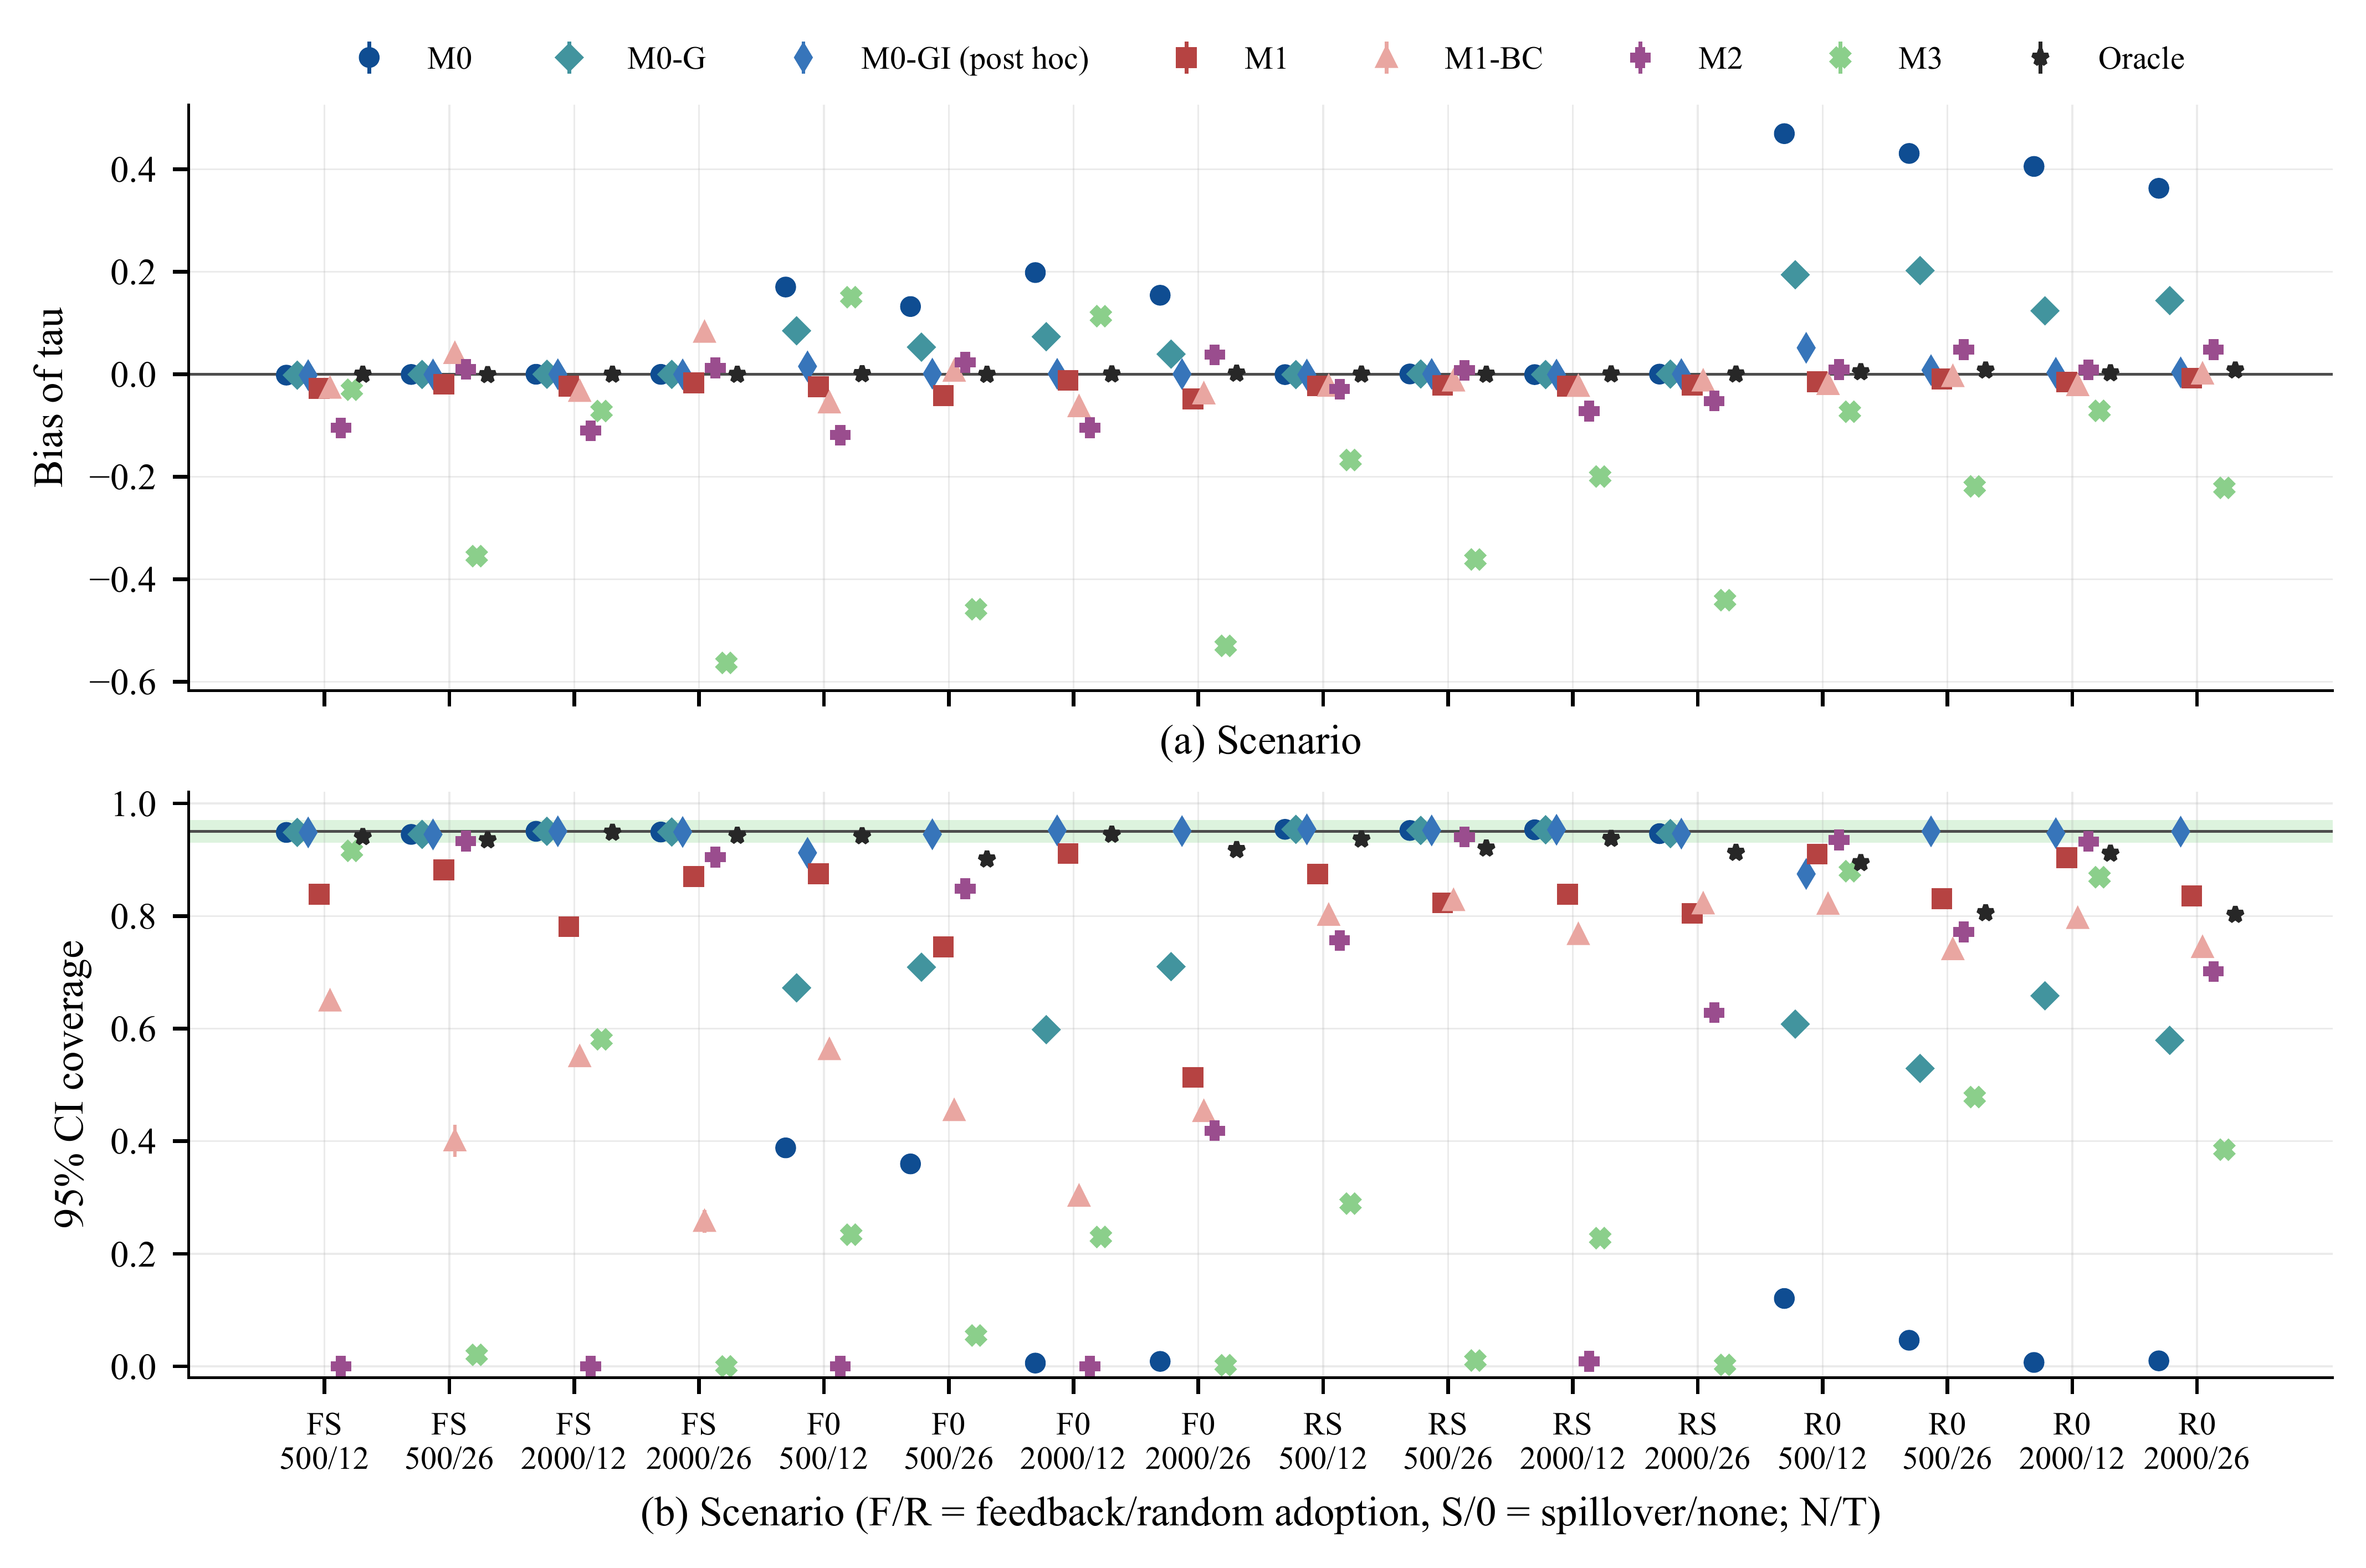
\includegraphics[width=\linewidth]{fig_01_core_tau.png}
\caption{16 个核心情景下的政策效应 $\tau$（$R=8000$）：(a) 偏倚（误差棒为 $\pm2$ MCSE）；(b) 95\% $t_{G-1}$ 区间覆盖率（阴影带为 93\%--97\%）。M0-GI 在相同数据集上事后评估。图内文字为英文，与英文稿图 1 相同。}
\label{fig:core-tau}
\end{figure}

在 $\tau_0=0$ 下，M0 与 M0-OI 的 $J$ 检验保持名义水平（分别为 4.7\% 到 5.2\% 与 4.4\% 到 4.9\%），M1 过度拒绝（6.3\% 到 9.7\%），M1-BC、M2 与 M3 更严重（网络表 3）。
正溢出下全部 8000 次重复都只有唯一根，M0、M0-G 与 M0-GI 结果相同。
$\phi_0=\kappa_0=0$ 位于定理~\ref{thm:asy} 之外，此时 47.2\% 到 51.7\% 的运行出现多个内部根，局部 M0 落入非相合根，偏倚为 0.132 到 0.469，覆盖率为 0.6\% 到 38.8\%（图~\ref{fig:roots}）。
第二个根是总体矩的性质：它出现在四个零传染设计的全部 40 个大 $N$ 抽样中，并随 $\bar\phi$ 移动（网络表 8）。
这些选根规则属于无理论保证的启发式方法。预试验后加入的 M0-G 在 28.6\% 到 44.8\% 的运行中选到 $\phi=0$（覆盖率 52.9\% 到 71.0\%），而事后不变性规则 M0-GI 在 63.7\% 到 80.9\% 的运行中选到边界，将偏倚降至 0.000--0.052、覆盖率提升至 87.5\%--95.2\%（表 2）。
在九个独立设计上（各 $R=2000$；网络附录 C.1），M0-GI 在 $\phi_0=0$ 处把覆盖率从 0.377 恢复到 0.893，但在 $\phi_0=0.05$ 处有 56\% 到 79\% 的运行选到边界，覆盖率从 0.960--0.970 降至 0.921--0.935；在 $\phi_0=0.15$ 处两条规则至多相差 0.001。

\begin{figure}[!t]
\centering
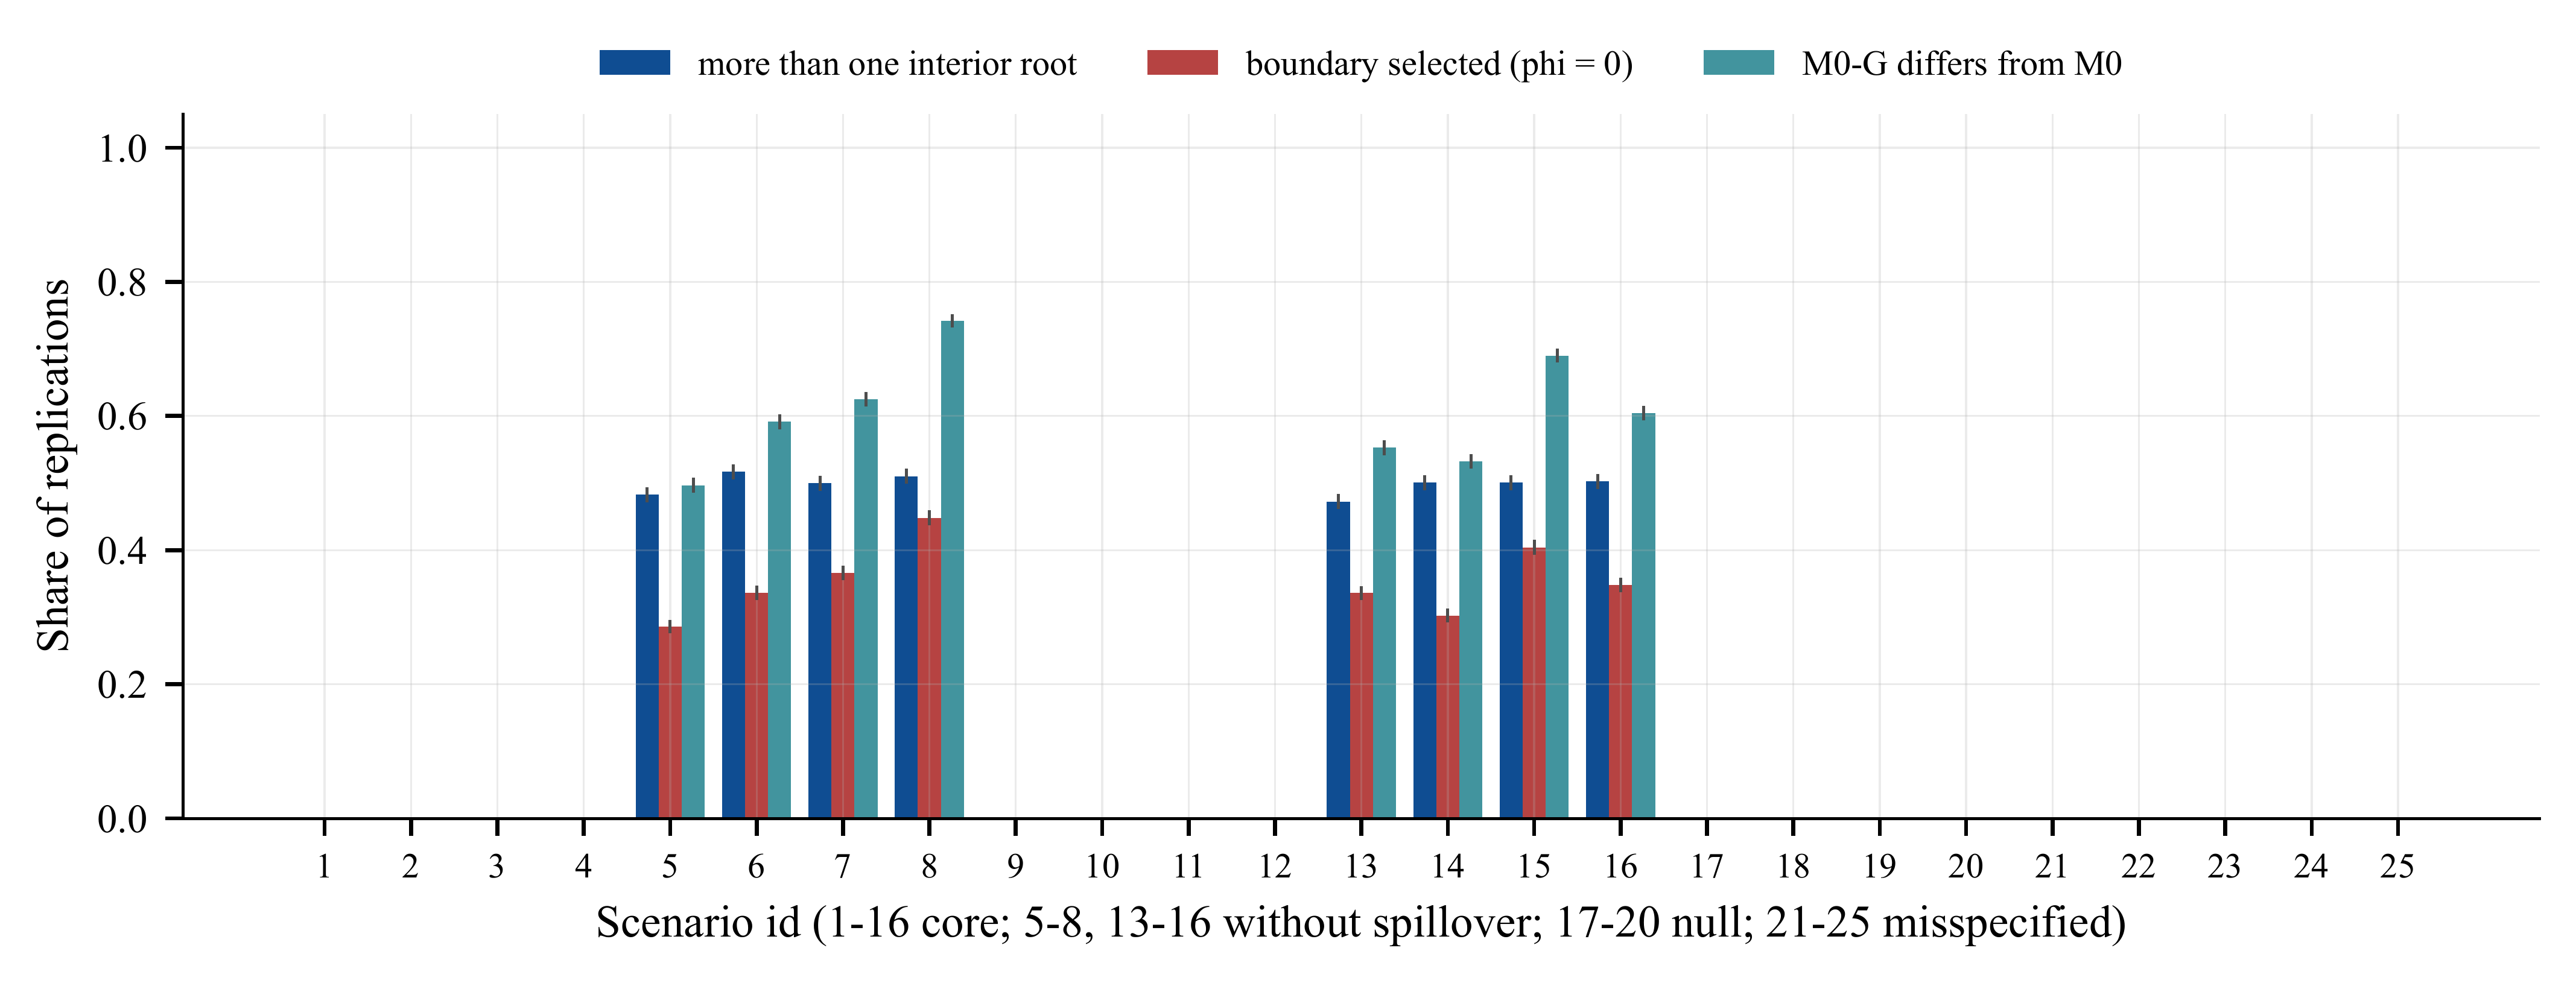
\includegraphics[width=\linewidth]{fig_02_roots.png}
\caption{$\phi\in[0,3]$ 上剖面 QD-GMM 的根诊断（$R=8000$，误差棒为 $\pm2$ MCSE）：出现多个内部根的比例、选到边界 $\phi=0$ 的比例，以及 M0-G 与 M0 不一致的比例。}
\label{fig:roots}
\end{figure}

动态累积效应下（X5），汇聚常数效应的 M0 失效（偏倚 0.219，覆盖率 0\%），事件时间规格 M0-ET 复原了每个分箱，覆盖率为 95.3\% 到 95.8\%（注~\ref{rem:dynamic}）。
代际权重错误（X1）几乎不影响 $\hat\tau$（偏倚 0.010，覆盖率 94.6\%），误差被 $\hat\phi$ 吸收（偏倚 $+0.516$）；实施后报告下降 15\%（X2）使 $\hat\tau+\hat\kappa$ 偏移约 $-0.35$；异质性（X3）与耗竭（X4）下 $\hat\tau$ 几乎无偏（网络表 5）。
有溢出时，实现的避免病例数 $\psi^\dagger$ 的相对偏倚中位数在受处理单元上位于 $\pm0.006$ 以内（全网络在 $\pm0.007$ 以内），$\psi^\dagger$ 区间覆盖率为 85.7\% 到 95.4\%；对总体 $\psi$ 的覆盖率为 72.1\% 到 92.5\%，因为区间不含过程噪声（注~\ref{rem:psi}；网络表 6）。

\subsubsection{周内传播}
\label{ss:sameweek}

主设计不含周内传染，A1 与 A4 严格成立。为在周内更新下单独考察周度聚合的影响（同周传递只发生在单元内部，A4 保持成立），本文在核心情景 $(N=500,T=12)$、反馈实施、$(\tau_0,\kappa_0,\phi_0)=(\log0.8,-0.1,0.4)$ 上模拟了两组种子独立的设计，各 $R=1000$ 次。
基准组为周度模型；同周组自窗口第 3 周起启用日度的单元内再感染，名义权重 $w_0=0.3$（再进入率 $g=1.744$；非线性再感染占总期望病例的 14.5\%，计入同周播种的发病为 34\%）。
基准组偏倚为 0.001（覆盖率 0.948）；同周更新使 $\hat\tau$ 偏倚 $-0.033$（MCSE 0.001，覆盖率 0.890），$\hat\kappa$ 偏倚 $-0.021$（0.002，覆盖率 0.939），$\hat\tau+\hat\kappa$ 偏倚 $-0.053$（0.002，覆盖率 0.783），约为真实总和的六分之一。
由于 A4 成立，夹心标准误保持校准，覆盖不足来自偏倚；$J$ 检验对此没有检验力（拒绝率 4.8\%，基准组 4.9\%）。去掉前三周后偏倚仍在（$-0.037$；网络附录 C）。
$w_0=0.3$ 的实验界定了周度聚合的适用边界：周度 QD-GMM 非常适用于代际间隔落在多周尺度、周内传播可忽略的病原体——如第~\ref{s:application} 节的水痘（$w_0<10^{-5}$）、麻疹或腮腺炎——而同周传播份额较大的快速代际病原体（如 SARS-CoV-2，$w_0\gtrsim 0.3$）则需要周内估计方程（网络附录 A.12）。

\section{应用：德国交错暑假与水痘县级传播压力测试}
\label{s:application}

\begin{figure}[!t]
\centering
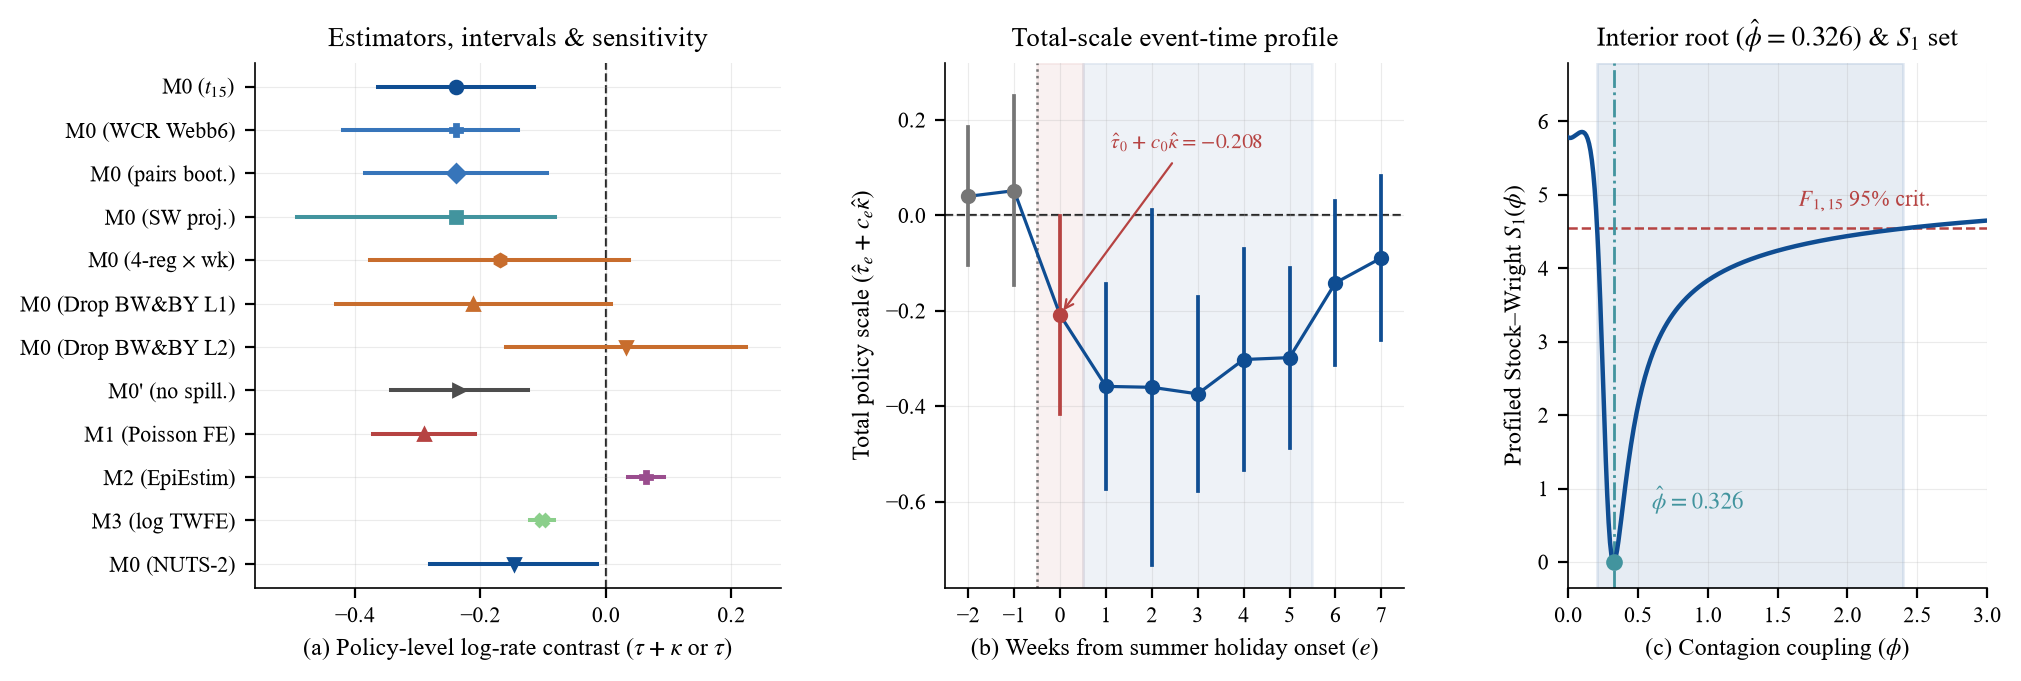
\includegraphics[width=\linewidth]{fig_03_application.png}
\caption{德国县级水痘压力测试（2015--2019 年，$N=400$，$G=16$ 州，$T=261$ 周）。(a) 各推断方法（$t_{15}$ 夹心、限制得分野 bootstrap-$t$ WCR Webb6、成对聚类 bootstrap-$t$ 与 Bonferroni 投影）、排除不轮换南部州、区域 $\times$ 周控制、全假期滞后 1 安慰剂、常用比较量（M0$'$、M1--M4）及 NUTS-2 聚合（$N=38$）下的政策层面效应及 95\% 区间。(b) 总政策尺度事件时间剖面 $\hat\tau_e+c_e\hat\kappa$（$e=-2,\dots,7$）：前趋势平缓（$e=-2,-1$）、起始周下降（$-0.208$）及开学后回升（$e=6,7$）。(c) $\phi\in[0,3]$ 上的剖面 Stock--Wright $S_1(\phi)$ 曲线，显示内部根 $\hat\phi=0.326$ 及 $F_{1,15}$ 95\% 置信集 $[0.21,2.40]$（阴影区）。}
\label{fig:app}
\end{figure}

例行学校假期与停课是研究呼吸道与儿童传染病传播的经典自然实验\citep{cauchemez2008school,jackson2014varicella,adda2016economic,isphording2021schools,vonbismarckosten2022schools}。与将观测估计视为干净因果基准不同，本文把 QD-GMM 应用于 2015--2019 年德国县级周度水痘（\emph{Windpocken}）监测面板，对估计量及整套内置诊断做蓄意压力测试。
水痘平均代际间隔约 14.0 天\citep{vink2014serial}，按周离散至滞后 $s=1,2,3$ 得 $w=(0.141,0.720,0.138)$（同周质量 $w_0=2.6\times 10^{-6}$），使生物学传播满足第~\ref{ss:sameweek} 节有效域，但以报告周（\emph{Meldewoche}）记录的数据仍可能受到假期就诊与申报延迟偏移的影响；14 个联邦州每年轮换暑假时间，而巴伐利亚州（BY）与巴登-符腾堡州（BW）长期固定于夏末（ISO 第 30--37 周）；此外 58.8\% 的县周为零计数（均值 1.10），构成了对定理~\ref{thm:bias} 的严苛检验。

监测数据取自罗伯特·科赫研究所 SurvStat@RKI 2.0\citep{faensen2006survnet}，涵盖全部 $N=400$ 县（柏林 12 区合并为单元 11000，无人口插补县）与 $T=261$ 周（2015-W01 至 2019-W52，共 115,129 例，另含 2014-W50--W52 三周前置样本；网络附录 D）。假期日历取自 OpenHolidays，县级邻接由 5 位 AGS 多边形构造（1,043 条无向边，平均度 5.22）。鉴于水痘约两周潜伏期及报告周口径，基准暴露 $D_{it}$ 采用过半周规则（该周至少 4 天处于暑假）并滞后一周（占县周 11.8\%）；$\ge 3$ 天（$-0.223$）、$\ge 5$ 天（$-0.190$）、连续比例（$-0.327$）及滞后 2 二值设定（$-0.331$，$[-0.714,0.052]$）见网络表 9。主推断按 $G=16$ 州聚类并采用 $t_{15}=2.13$ 及有限簇校正确认。

\subsection{基准估计、比较量与非轮换州敏感性}

因暑假设在州层面，内陆县 $D_{it}=\bar D_{it}$，直接可识别对比为政策层面总量 $\tau+\kappa$。基准 M0（$\bar\phi=0.5$）给出 $\hat\tau+\hat\kappa=-0.239$（SE $0.0584$；95\% $t_{15}$ 区间 $[-0.364,-0.115]$），即工作模型下传播率下降 21.3\%，分量估计为 $\hat\tau=-0.300$（$[-0.854,0.254]$）、$\hat\kappa=0.060$（$[-0.538,0.659]$）、$\hat\phi=0.326$（SE $0.0567$，$[0.205,0.446]$）。在基准 $\omega_i=\text{人口}_i/10^5$ 下反事实传播对应暑期减少 2,453 例（SE 673）、全网减少 3,012 例（SE 904），但高度依赖 $\omega_i$ 尺度（$\omega_i\times 0.25$ 为 5,355 / 15,615 例；$\omega_i\times 4.0$ 为 1,585 / 1,633 例，因 $\hat\phi$ 随 $\omega_i$ 由 0.618 移至 0.037）。

常用比较量直接印证了定理~\ref{thm:bias}：县级 58.8\% 零计数下两步 EpiEstim 对数 $R$（M2）反号为 $+0.064$（$[0.036,0.093]$），聚合至 38 个 NUTS-2 区域（零计数降至 2.9\%）后 M0 仍为 $-0.147$（$[-0.280,-0.013]$）而 M2 立即反转为 $-0.102$（$[-0.140,-0.065]$）；$\log(Y+1)$ TWFE（M3）衰减至 $-0.102$，M1/M4 将 $\hat\phi$ 压塌至 0.058 与 0.001。

然而，M0 的 $-0.239$ 对比在控制南部非轮换州或细分区域季节性后明显脆弱（网络表 10）。加入东/西德 $\times$ 周效应得 $-0.217$（$[-0.323,-0.112]$），加入州线性趋势得 $-0.315$（$[-0.471,-0.160]$），州单谐波季节曲线得 $-0.224$（$[-0.371,-0.077]$），但同时剔除从不轮换的 BW 与 BY（$N=260, G=14$）后滞后 1 估计缩至 $-0.211$（区间 $[-0.431,0.008]$ 包含零）、滞后 2 反号为 $+0.033$（$[-0.158,0.224]$）；四大区 $\times$ 周固定效应同样使滞后 1 缩至 $-0.169$（$[-0.376,0.038]$）、滞后 2 至 $-0.072$（$[-0.348,0.204]$），反映单纯轮换日历难以分离夏末季节低谷与南部水痘疫苗接种差异\citep{siedler2010varicella,reuss2010varicella}。

\subsection{少簇推断、多根检验与过度识别}

在校准 400 县 $\times$ 261 周模拟中（每组 $R=500$；网络附录 E），1,000/1,000 次均收敛至唯一内部根（偏倚 $-0.003$），但因 $G=16$ 州规模悬殊，夹心标准误低估抽样标准差 14.5\%（SE 比值 $0.855$，高噪声 $0.830$），使 $t_{15}$ 覆盖率为 0.902（高噪声 0.904），非限制线性能得分 bootstrap 亦偏窄（Mammen 0.872、Webb6 0.894）。施加原假设的限制得分野 bootstrap（WCR-score；\citealp{kline2012score}）将覆盖率恢复至 0.936（Webb6）与 0.934（Rademacher；高噪声 0.946），在德国观测数据上给出更宽的 95\% 区间（$[-0.419,-0.139]$ 与 $[-0.429,-0.119]$，$p=0.002/0.003$），与成对聚类 bootstrap-$t$（$[-0.385,-0.094]$）及删一州刀切（$[-0.375,-0.104]$，留一范围 $[-0.269,-0.203]$）吻合。计入 29 对邻近州得分交叉项（注~\ref{rem:testable}）在 $G=16$ 下得到非正定协方差矩阵（最小特征值 $-0.020$，$\tau,\kappa$ 方差为负）。

满秩得分过度识别诊断显示出明确的工作模型设定张力：虽然 $[0,3]$ 剖面仅有一处内部根 $\hat\phi=0.326$，且 $S_{3,\mathrm{inv}}$ 选择内部根（4.26 对 8.67），$S_{3,\mathrm{oi}}$ 却微弱偏向 $\phi=0$ 边界（9.113 对 9.120），使 M0-G 落在边界上。参考值不变性通过（$J_{LM,\mathrm{inv}}=4.10$，$p_F=0.184$，校准 $p=0.088$），但滞后工具检出显著拒绝：$J_{LM,\mathrm{oi}}=9.12$（$p_F=0.036$，校准 $p=0.004$ vs.\ 第 95 分位数 5.33），其来源单一集中于一周滞后对数增长矩（$6.74$，$p_F=0.020$），滞后输入压力份额通过（$1.13$，$p_F=0.304$）。Stock--Wright 统计量在 $\bar\phi=0.5$ 下给出 $S_1(0)=5.78$（$p_F=0.030$）与连通 $S_1(F)$ 集 $[0.21,2.40]$（Bonferroni 投影 $[-0.493,-0.081]$），但过度识别 $\chi^2$ 集 $S_{3,\mathrm{oi}}(\chi^2)$ 在全部三个 $\bar\phi$ 下均为空集，而 $F_{3,14}$ 校准下的 $S_{3,\mathrm{oi}}(F)$ 与 $S_{3,\mathrm{inv}}(F)$ 均覆盖完整网格 $[0.00,3.00]$。

\subsection{报告时序、短期假期安慰剂与识别边界}

把事件时间系数改写到政策总效应尺度 $\hat\tau_e+c_e\hat\kappa$ 后（图~\ref{fig:app}(b)，网络表 14）：前趋势平缓（$e_{-2}=+0.040$，$e_{-1}=+0.052$；联合 $p_F=0.765$），但在放假起始周 $e_0$ 即出现 $-0.208$（SE $0.097$，$p=0.049$，CI $[-0.416,-0.001]$）的急剧下降，随后 $e_1$--$e_5$ 为 $-0.298$ 至 $-0.374$，开学周 $e_6,e_7$ 回升至 $-0.141$ 与 $-0.089$（联合 $p_F=0.172$）。按水痘约 14 天代际间隔，起始当周 $-0.208$ 降幅反映假期首周就诊与报告压缩。

报告率临界点与安慰剂检验进一步印证了这一点（网络表 15 与 16）：若按同期报告暴露 $D_{it}^{(0)}$ 匹配零起始周下降，需 21.5\% 的暑期申报下降，而该校准直接把滞后 1 基准估计推回 $+0.007$（SE $0.063$）、滞后 2 为 $-0.213$（覆盖零）。复活节、秋季、冬季与圣灵降临节等非暑期短期假期均在滞后 0 呈现显著负降（$-0.198$ 至 $-0.497$），并在滞后 2 出现正向回补（复活节 $+0.241$ $[0.119,0.363]$，秋季 $+0.150$ $[0.054,0.247]$）；全部假期指标在滞后 1 缩至 $-0.081$（$[-0.183,0.021]$）。尽管 200 次跨州随机置换（均值 $0.000$，SD $0.089$）证实观测 $-0.239$ 位于极端尾部（双侧 $p=0.010$），说明该效应特异跟随各州暑假排期，但报告周数据本身无法剥离生物学传播变化与假期申报/出行波动。

\section{讨论}
\label{s:discussion}

把平行趋势放在带输入感染压力的对数再生数上，并用前向准差分消去不受限制的单元效应，得到了一套同时容纳自我激发传播、发病驱动政策反馈与滞后空间传染的双重差分设计，同时保留闭式周剖面解与常规聚类稳健夹心方差。
在涵盖反馈、溢出、过度离散与小计数的 25 个预设模拟情景中，QD-GMM 几乎无偏且覆盖率达名义水平，而结局尺度、泊松固定效应与两步再生数比较量均出现系统性偏倚；当政策设在报告单元之上时，设计直接识别政策层面总效应 $\tau+\kappa$。

将框架应用于德国 2015--2019 年县级水痘监测面板，既检验了理论预测，也清晰标定了工作模型诊断所能揭示的实证边界。
一方面，58.8\% 县周零计数下两步 EpiEstim 对数 $R$ 回归即刻反号（县级 $+0.064$ 对 NUTS-2 聚合 $-0.102$）、$\log(Y+1)$ TWFE 严重衰减至 $-0.102$，直接验证了定理~\ref{thm:bias}，而 QD-GMM 无需删零并复原了内部耦合参数 $\hat\phi=0.326$。
另一方面，诊断套组阻止了把基准 $-0.239$ 解释为干净的 21.3\% 生物学因果减毒效应：（i）识别高度依赖从不轮换的巴伐利亚与巴符州（同时剔除后滞后 1 缩至 $-0.211$ $[-0.431,0.008]$、滞后 2 转正 $+0.033$），且四大区 $\times$ 周控制吸收大部分轮换变异；（ii）滞后工具检验显著拒绝（$J_{LM,\mathrm{oi}}=9.12$，$p_F=0.036$，校准 $p=0.004$），$S_{3,\mathrm{oi}}$ 偏向边界且 $S_{3,\mathrm{oi}}(\chi^2)$ 为空集；（iii）SurvStat@RKI 按报告周记录病例，总尺度起始周急降（$-0.208$）及短期假期先降后弹（lag 0 负降、lag 2 正补）显示假期申报压缩与补报共存。

周度 QD-GMM 的实际适用由三个条件界定。第一是根唯一性与诚实诊断披露：应剖面检查 $[0,3]$，将 M0-G/M0-GI 与 Stock--Wright 识别稳健集\citep{stock2000weak}配套报告，并把 $J_{LM,\mathrm{oi}}$ 拒绝或空 $\chi^2$ 集视为明确的工作模型警示。
第二是时间聚合与报告口径：同周实验（$w_0=0.3$，第~\ref{ss:sameweek} 节）表明周度 QD-GMM 要求多周代际间隔且报告偏移平稳；快速代际病原体或受假期就诊波动影响的报告周序列需要纳入星期与延迟结构的周内估计方程\citep{lison2024nowcast}。
第三是有限簇推断：$G=16$ 校准模拟显示 $t_{15}$ 对 $\tau+\kappa$ 覆盖率仅为 0.902、非收缩邻近州校正可呈非正定，因此簇数适中时应配合限制得分野 bootstrap（WCR-score）、成对聚类 bootstrap 与删一簇刀切\citep{kline2012score,mackinnon2017wild,ferman2019inference,canay2021wild}。

在对数再生数尺度上建立平行趋势\citep{roth2023parallel}将本地与输入感染压力分开\citep{elenev2025staggered}，并与无混杂性框架\citep{callaway2023pandemic}互补。序贯效率界\citep{chamberlain1992sequential,chamberlain2022feedback}、似然反馈模型\citep{bonhomme2025feedback}、周内估计方程、不依赖报告的污水监测信号\citep{goldstein2024wastewater}以及联合估计代际间隔、免疫接种与报告过程\citep{siedler2010varicella,suzuki2023varicella,goldwasser2026rt}均是自然延伸。

\section*{致谢}
\markboth{声明}{声明}
作者感谢罗伯特·科赫研究所（SurvStat@RKI 2.0）、OpenHolidays 项目（整理德国文教部长会议官方学校假期日历）以及德国行政区划开放地理数据维护者公开监测、假期与地理记录。

\section*{数据可得性声明}
所有数据均公开可得；来源、查询条件、校验和与可运行下载脚本（\path{experiment/data/fetch_germany.py}）见网络附录 D 与 \texttt{experiment/data}。完整复现代码随文提供。

\section*{支持材料}
网络附录 A--F（正则条件、证明与改写的比较量结果、数值核对、补充模拟、数据来源与清洗、少簇推断、应用诊断）在第~\ref{s:intro}--\ref{s:discussion} 节中引用，作为本文的支持材料提供。

\section*{利益冲突}
作者声明无利益冲突。

\section*{资助}
（资助声明待投稿前补充。）

\appendix
\section*{网络附录（对应英文稿 Web Appendix A.9--A.12）}
\addcontentsline{toc}{section}{网络附录（对应英文稿 Web Appendix A.9--A.12）}
\markboth{网络附录 A.9--A.12}{网络附录 A.9--A.12}
\setcounter{section}{0}
\setcounter{equation}{0}
\renewcommand{\theequation}{A.\arabic{equation}}

\subsection*{A.9 反馈下常用估计量估计的是什么}
\addcontentsline{toc}{subsection}{A.9 反馈下常用估计量估计的是什么}
\label{ss:bias}

(a)--(c) 部分取 $\kappa_0=\phi_0=0$，并把压力 $\Lambda_{it}=L_{it}+\omega_i$ 视为已知，这对比较方法有利。$\ddot D_{it}$ 表示平衡面板中双向去均值的 $D_{it}$，$d^2=\lim N^{-1}\E\sum_{i,t}\ddot D_{it}^2>0$，极限在 $T$ 固定、$G\to\infty$ 下取。

\begin{theorem}[伪真值]
\label{thm:bias}
假设 A1--A6 与 (L)。
\begin{enumerate}[leftmargin=2em,label=(\alph*)]
\item \emph{两步对数 $R$ 双重差分。} 设 $\hat\tau_2$ 为 $y_{it}=\log\{(Y_{it}+c)/\Lambda_{it}\}$ 对 $D_{it}$ 的双向固定效应斜率，$c>0$\citep{feng2024parallel}。
令 $b_{it}=\log\mu_{it}-\E\{\log(Y_{it}+c)\mid\F_{t-1}\}$，$\eta_{it}=\log(Y_{it}+c)-\E\{\log(Y_{it}+c)\mid\F_{t-1}\}$。则精确地有 $\hat\tau_2-\tau_0=\{-\sum\ddot D_{it}b_{it}+\sum\ddot D_{it}\eta_{it}\}/\sum\ddot D_{it}^2$，且 $\hat\tau_2\to_p\tau_0+B_J+B_F$，其中各项如下：
\[
B_J=-\lim\frac{\E\sum_{i,t}\ddot D_{it}b_{it}}{Nd^2},\qquad
B_F=-\lim\frac{\E\sum_i\sum_{t<s}D_{is}\eta_{it}}{NTd^2},\qquad
|B_F|\le\frac{2\bar\sigma_\eta T^{1/2}}{3d^2},
\]
$(\bar\sigma_\eta)^2=\sup_{i,t}\E\eta_{it}^2$。在均值为 $\mu$、形状为 $k$ 的负二项工作分布下，二阶展开给出 $b_{it}\approx-(c-1/2+c/k)/\mu_{it}+1/(2k)$。若 $\E(\eta_{it}\mid D_{i1},\dots,D_{iT})=0$ 则 $B_F=0$；实施跟随异常高的病例时 $B_F<0$。
\item \emph{泊松固定效应。} 设 $\hat\beta_1$ 为以 $\log\Lambda_{it}$ 为偏移、含单元与周效应、回归元为 $x_{it}$ 的条件（泊松固定效应）估计量。其估计函数为 $S_i(\beta)=\sum_s\{x_{is}-\bar x^m_i(\beta)\}Y_{is}$，$\bar x^m_i=\sum_s m_{is}x_{is}/\sum_s m_{is}$，且 $\E S_i(\beta_0)=-\sum_s\E\{\bar x^m_i(\beta_0)\varepsilon_{is}\}$；当 $\Lambda_{i,s+1}$ 或 $D_{i,s+1}$ 依赖 $Y_{is}$ 时，该量一般不为零。
若 $Y_{is}\mid\F_{s-1}$ 为泊松分布，且 $\bar x^m_i=f(Y_{is},R_{is})$，$R_{is}$ 条件独立于 $Y_{is}$，则 $\E(\bar x^m_i\varepsilon_{is}\mid\F_{s-1})=\mu_{is}\E\{f(Y_{is}+1,R_{is})-f(Y_{is},R_{is})\mid\F_{s-1}\}$\citep{chen1975poisson}。
取 $T=2$、$S=1$、$D_{i1}=0$，$D_{i2}$ 为 $Y_{i1}$ 与独立噪声的函数，组 $D_{i2}=d$ 中伪真的第 2 周对数增长 $\tilde h_d$ 满足下式：
\begin{equation}
\E\Bigl[\ind(D_{i2}=d)\,\Lambda_{i2}\,\frac{\Lambda_{i1}e^{\alpha_i+h_0+\tau_0d}-e^{\tilde h_d}Y_{i1}}{\Lambda_{i1}+e^{\tilde h_d}\Lambda_{i2}}\Bigr]=0,
\label{eq:t2fe}
\end{equation}
且 $\hat\tau_1\to_p\tilde h_1-\tilde h_0$。由于 $\Lambda_{i2}=Y_{i1}+\omega_i$，一般有 $\tilde h_d\ne h_0+\tau_0d$，从而 $\tilde h_1-\tilde h_0\ne\tau_0$，即使 $D_{i2}$ 是随机化的。
\item \emph{$\log(Y+1)$ 上的双向固定效应。} 斜率 $\hat\tau_3$ 满足下式：
\[
\hat\tau_3-\tau_0=\frac{\sum\ddot D_{it}\log\Lambda_{it}}{\sum\ddot D_{it}^2}+\frac{-\sum\ddot D_{it}b^{(1)}_{it}+\sum\ddot D_{it}\eta^{(1)}_{it}}{\sum\ddot D_{it}^2},
\]
其中 $b^{(1)},\eta^{(1)}$ 取 (a) 中 $c=1$ 的形式。第一项来自省略的压力，实施跟随压力上升时为正，政策压低后续压力时为负，偏倚符号因此不确定。
\item \emph{忽略溢出。} 设 $(\tilde\delta,\tilde\tau)$ 是强加 $\kappa=\phi=0$、使用工具 $s_{it}e_t$ 与 $s_{it}D_{it}$ 的 QD-GMM 的伪真值，它满足 $\lim G^{-1}\E\sum_{i,t}z_{it}\mu_{it}\{R_{it}(\delta,\tau)-1\}=0$，其中的比值如下：
\[
R_{it}(\delta,\tau)=\exp\{\gamma_{t+1}-\gamma_t-\delta_t-(\tau-\tau_0)\Delta D_{i,t+1}+\kappa_0\Delta\bar D_{i,t+1}\}\,\frac{1+\phi_0\tilde N_{i,t+1}}{1+\phi_0\tilde N_{it}},
\]
$\tilde N_{it}=N_{it}/(L_{it}+\omega_i)$，$\Delta X_{i,t+1}=X_{i,t+1}-X_{it}$。若 $\kappa_0=\phi_0=0$ 则 $\tilde\tau=\tau_0$。
在 $(\kappa_0,\phi_0)$ 的一阶上，$\tilde\tau-\tau_0$ 等于以 $s_{it}\mu_{it}$ 为权重、以 $(e_t,D_{it})$ 为工具，把 $\kappa_0\Delta\bar D_{i,t+1}+\phi_0\Delta\tilde N_{i,t+1}$ 对周指示与 $\Delta D_{i,t+1}$ 做恰好识别工具变量回归时 $\Delta D_{i,t+1}$ 的系数。当 $\Delta\bar D$ 随 $\Delta D$ 一起变动（如州级实施）时，$\kappa_0$ 的贡献与 $\kappa_0$ 同号。
\end{enumerate}
\end{theorem}

定理~\ref{thm:bias} 把计数面板中前定回归元的已知结果改写到更新均值上，作用是把各比较方法放在同一框架下比较，不建立新的不相合结果。
(a) 部分把两种机制分开。Jensen 项 $B_J$ 是估计再生数的小计数问题，不随 $T$ 增大而消失；反馈项 $B_F$ 的来源是 $D$ 的单元均值用到了未来的实施，而未来实施对当期冲击有反应，这正是动态面板中组内估计量固定 $T$ 偏倚的机制\citep{nickell1981biases}。
由于 $d^2$ 对全部 $t=1,\dots,T$ 求和，在每期单元内处理变异不消失的设计中 $d^2$ 随 $T$ 线性增长，(a) 中的一般上界因此为 $O(T^{-1/2})$；在近期冲击条件下交叉乘积和为 $O(T)$，上界 $C/d^2$ 为 $O(T^{-1})$，与 Nickell 速率一致。
(b) 部分说明回归元（这里是滞后结局偏移）为前定而非严格外生时泊松固定效应估计量经典的固定 $T$ 不相合\citep{hausman1984count,wooldridge1997multiplicative,wooldridge1999distribution,blundell2002count}；它在随机化实施下同样成立，但在网络附录 B 的随机化设计中偏倚为 $-0.004$，因此 (b) 在那里是示例，没有实际影响。
(c) 部分是\citet{santossilva2006log} 与\citet{chen2024logs} 的对数线性化问题再加上省略的压力项；基于泊松的双重差分\citep{wooldridge2023nonlinear}消除前者，不能消除后者。
分面板刀切校正\citep{dhaene2015splitpanel}依赖平稳性，周效应与交错实施都违背平稳性；大 $N$、大 $T$ 非线性面板的解析校正\citep{fernandezval2016individual}需要长面板，因此校正后的估计量只用模拟评估。

\subsection*{A.10 异质效应与动态效应}
\addcontentsline{toc}{subsection}{A.10 异质效应与动态效应}

\begin{proposition}[异质效应]
\label{prop:hetero}
设 A1 成立，但效应为单元特定、时不变的 $\tau_i$，可以与 $\alpha_i$ 及实施过程相关；实施为吸收式，$(\kappa,\phi)=(\kappa_0,\phi_0)$ 固定，使用定理~\ref{thm:ident}(b) 的工具。
令 $M_t=\lim G^{-1}\E\sum_i s_{it}\mu_{it}$，并设有某个 $t$ 使 $A_t>0$、$K_t>0$。则伪真值 $\tilde\tau$ 存在且唯一，落在 $\tau_i$ 支撑集在度量 $s_{it}\mu_{it}\Sw_{i,t+1}$（限于 $A_t>0$ 的周）下的闭凸包内。在 $\tau_i-\tilde\tau$ 的一阶上有如下近似：
\[
\tilde\tau\approx\frac{\sum_t(A_t/M_t)\lim G^{-1}\E\sum_i s_{it}\mu_{it}\Sw_{i,t+1}\tau_i}{\sum_t(A_t/M_t)K_t}.
\]
这是一个权重非负的加权平均。
\end{proposition}

命题~\ref{prop:hetero} 把交错实施下双向固定效应的加权分析\citep{goodmanbacon2021did,dechaisemartin2020twfe}改写到准差分矩上；它把 $(\kappa,\phi)$ 固定在真值，权重为一阶近似。
效应时不变时，常数效应的 QD-GMM 估计目标不会给任何单元的效应赋负权重，这一点与双向固定效应不同。没有受处理单元的周里的切换者一阶权重为零。

\setcounter{remark}{1}
\begin{remark}[动态效应]
\label{rem:dynamic}
若效应随实施后时间变化，已处理的维持者不再消去 $\tau$，它们的病例增长中含有 $\tau_{e+1}-\tau_e$。由于已处理单元参与钉住周效应（命题~\ref{prop:sources}），常数效应估计目标可能落在真实效应范围之外，甚至符号相反，与双向固定效应中的已处理比较问题相同\citep{goodmanbacon2021did}。
因此本文推荐事件时间规格 $\sum_{e=0}^{E}\tau_e\ind\{t-A_i=e\}$，其中 $A_i$ 为实施周，最后一格汇总 $e\ge E$，以 $s_{it}\ind\{t-A_i=e\}$ 为工具。这些指示变量是 $\F_{t-1}$ 可测的，只要秩条件成立，定理~\ref{thm:asy} 即适用。秩条件要求存在尚未处理或从未处理的单元。
\end{remark}

注~\ref{rem:dynamic} 把\citet{sun2021estimating} 与\citet{borusyak2024imputation} 的事件研究分析改写到准差分矩上。隐含权重可以写成显式形式。
设事件时间模型成立，分箱效应为 $\tau^*=(\tau^*_0,\dots,\tau^*_E)^{\top}$；当政策以分箱系数 $\boldsymbol\tau$ 进入时，记汇聚恰好识别矩（剖面消去周效应）的极限为 $\bar g_P(\boldsymbol\tau,\kappa,\phi)$，汇聚规格取 $\boldsymbol\tau=\tau\mathbf 1$。
汇聚伪真值 $(\tilde\tau,\tilde\kappa,\tilde\phi)$ 满足 $\bar g_P(\tilde\tau\mathbf 1,\tilde\kappa,\tilde\phi)=0$。在 $(\tau^*,\kappa_0,\phi_0)$ 处记 $H_b=\partial\bar g_P/\partial\boldsymbol\tau^{\top}$、$H_\kappa=\partial\bar g_P/\partial\kappa$、$H_\phi=\partial\bar g_P/\partial\phi$，一阶展开给出如下关系：
\[
A\,(\tilde\tau,\ \tilde\kappa-\kappa_0,\ \tilde\phi-\phi_0)^{\top}=H_b\tau^*,\qquad
A=[H_b\mathbf 1,\ H_\kappa,\ H_\phi].
\]
于是 $\tilde\tau\approx\sum_{b}\omega_b\tau^*_b$，$\omega^{\top}$ 为 $A^{-1}H_b$ 的第一行。由于 $A^{-1}H_b\mathbf 1=e_1$，权重之和为一；已处理的维持者在 $H_b$ 中与切换者符号相反，权重因此可以为负。
第二行表明分箱效应不同时 $\tilde\kappa$ 也受到污染。网络表 14 报告第~\ref{s:application} 节应用中围绕暑假起始周的动态事件时间剖面。

\subsection*{A.11 避免病例数}
\addcontentsline{toc}{subsection}{A.11 避免病例数}

令 $t\le 0$ 时 $\nu_{it}=Y_{it}$。对 $t\ge 1$，反事实在所有单元上联合递推定义如下：
\begin{equation}
\nu_{it}(\theta)=c_{it}(\theta)Y_{it},\qquad
c_{it}(\theta)=e^{-\tau D_{it}-\kappa\bar D_{it}}\,\frac{\Lambda_{it}(\nu;\phi)}{\Lambda_{it}(Y;\phi)},
\label{eq:nu}
\end{equation}
其中 $\Lambda_{it}(\nu;\phi)$ 是由 $\nu$ 算出的压力。在政策直接作用、经由 $\bar D_{it}$ 或经由所受压力影响单元 $i$ 之前，递推保持 $\nu_{it}=Y_{it}$，因此无需选择反事实的起始日。
令 $\hat\psi_{\mathcal P}=\sum_{(i,t)\in\mathcal P}\{\nu_{it}(\hat\theta)-Y_{it}\}$，$\psi^\dagger_{\mathcal P}=\sum_{(i,t)\in\mathcal P}\{\nu_{it}(\theta_0)-Y_{it}\}$。

\begin{theorem}[反事实传播]
\label{thm:psi}
(a) 在 A1--A3 与 A5 下，对所有 $i$、$t$ 有 $\E(\nu_{it}(\theta_0)\mid\alpha,Y_{\le 0})=\E\{Y_{it}(\mathbf 0)\mid\alpha,Y_{\le 0}\}$，故 $\E\psi^\dagger_{\mathcal P}=\psi_{\mathcal P}$。
(b) 在定理~\ref{thm:asy} 的条件下，若 $|\mathcal P|/G$ 有界且 $\partial\nu_{it}/\partial\beta$ 满足网络附录 A.1 的控制条件，则 $G^{1/2}(\hat\psi_{\mathcal P}-\psi^\dagger_{\mathcal P})/G\to_d N(0,\Psi V\Psi^{\top})$，其中 $\Psi=\plim G^{-1}\sum_{(i,t)\in\mathcal P}\partial\nu_{it}(\theta_0)/\partial\theta^{\top}$。
\end{theorem}

直接按 $Y_{it}e^{-\tau D_{it}-\kappa\bar D_{it}}$ 缩放忽略了被避免的病例本身也会传染他人；定理~\ref{thm:psi} 让反事实沿更新方程与网络传播。(b) 部分是定理~\ref{thm:asy} 的标准 delta 方法推论，不含新的渐近论证。(b) 中的推断针对实现路径上的量 $\psi^\dagger$，其期望为 $\psi$。

\begin{remark}[过程噪声与耗竭]
\label{rem:psi}
$\psi^\dagger_{\mathcal P}-\psi_{\mathcal P}$ 是零均值、局部相关项之和。与矩贡献不同，这些项在相邻集群间相关，因为 $\nu_{it}$ 依赖邻居的结局。总体水平 $\psi_{\mathcal P}$ 的方差估计量需要加入集群图 HAC 项；本文推测其相合，但未给出证明。
若易感者耗竭使 A1 中的均值乘以 $1-C_{i,t-1}/P_i$（$C$ 为累计病例，$P$ 为人口），递推不再关于过去的 $\nu$ 线性，定理~\ref{thm:psi}(a) 只近似成立；耗竭还会使效应估计随暴露时间漂移\citep{janvin2025depletion}。
\end{remark}

\begin{remark}[可检验性]
\label{rem:testable}
引理~\ref{lem:mds} 意味着相邻集群的矩贡献不相关，这一点可以直接核对。应用中，29 对相邻德国联邦州的得分贡献相关系数为 0.175（$\tau$）、0.119（$\kappa$）与 $-0.123$（$\phi$）；把相邻对交叉乘积加入 $\hat\Omega$ 后，所得协方差矩阵非半正定（最小特征值 $-0.020$，$\tau$ 与 $\kappa$ 方差元为负值），尽管 $\hat\tau+\hat\kappa$ 与 $\hat\phi$ 的形式二次型分别由 0.0584 与 0.0567 降至 0.0482 与 0.0352，但非半正定修正矩不能支持“常规夹心方差偏保守”的结论（且与网络表 11 中夹心标准误低估约 16\% 的校准模拟一致）。
推论~\ref{cor:J} 的 $J$ 检验沿用\citet{arellano1991tests} 的思路，用额外的前定工具核对乘性更新结构；把 $D$ 滞后一周的敏感性分析核对政策时点对齐。
序贯可忽略性（A2(b)）与实施后未处理对数传播路径的平行性不可检验：反馈下前导回归不是有效检验（命题~\ref{prop:sources}(c)），预检验会扭曲后续推断\citep{roth2022pretest}；允许有界偏离平行趋势的方法\citep{rambachan2023credible}与基于设计的动态效应视角\citep{bojinov2021panel}是可选的替代，本文未采用。
\end{remark}

\subsection*{A.12 周内传播与假设 A4}
\addcontentsline{toc}{subsection}{A.12 周内传播与假设 A4}
\label{ss:weekwithin}

A4 要求给定历史后，同一周内各集群的结局相互独立。若一次感染在同一周内跨过集群边界，且两县都在该周被记录，则给定 $\F_{t-1}$ 时第 $t$ 周的两个新息相关，A4 恰好在关键之处失效。下文讨论这种情形何时出现以及代价多大。

A4 约束的是新息，不约束结局水平。相邻集群通过 $\bar D$ 和网络压力 $\Lambda$ 共享历史，引理~\ref{lem:mds} 以 $\F_{s-1}$ 可测因子对每个矩贡献加权，已经计入这一层。A4 排除的是与结局同一周到达、来不及进入信息集的相关。

周面板只有在传染至少滞后一期时才内在一致，因为定义估计目标的更新方程 \eqref{eq:mean} 按整周书写。同周传播改变该模型隐含的条件均值，也可能改变准差分的协方差结构；所得的矩未必仍是鞅差，相合性论证和常规聚类夹心方差在没有附加条件时都不能沿用。参数与方差偏差的方向和大小不能仅由周度模型确定。
对 SARS-CoV-2 等快速代际病原体，约 30\% 的传播落在同一周；第~\ref{ss:sameweek} 节的匹配模拟生成单元内周内更新（$w_0=0.3$，非线性周内再感染占 14.5\%）并聚合到周，周估计量偏倚约为真实效应的 15\%，$\tau$ 与 $\tau+\kappa$ 覆盖率分别降至 0.89 与 0.78，$J$ 检验检不出这一误设。相比之下，第~\ref{s:application} 节的水痘同周份额不足 $10^{-5}$（$w_0=2.6\times 10^{-6}$），周内聚合偏倚可忽略。

同周传播造成的依赖可以在下一期信息集建立之前把不同集群的新息联系起来。这与 A4 和引理~\ref{lem:mds} 允许的滞后跨集群传播不同；现有条件不能推出所得矩贡献在工具半径之外仍不相关。\citet{conley1999gmm} 那样的空间校正在相应依赖条件下处理协方差，但它本身不能修复误设的条件均值，也不能恢复鞅差性质。
25 个预设情景不含同周传播；第~\ref{ss:sameweek} 节的匹配模拟单独量化了它对偏倚与覆盖率的影响。

当相当比例的传播发生在一周之内时，周度聚合可能不够。缩短观测间隔或设定周内更新过程会改变数据模型：日计数带有星期报告效应与报告延迟\citep{lison2024nowcast}，违反命题~\ref{prop:ascertainment} 的无延迟报告，需要新的矩条件和新的模拟验证。仅靠方差校正无法解决均值设定问题，因此同周份额较大的快速代际病原体（$w_0\gtrsim 0.3$）需要专用的周内估计量。

同周模拟中，周内机制自从零计数的窗口序号 2（\texttt{ENGINE\_FROM = 2}）即窗口第 3 周起启用。

\section*{网络附录 D：数据来源与清洗}
\addcontentsline{toc}{section}{网络附录 D：数据来源与清洗}
\markboth{网络附录 D}{网络附录 D}

应用使用存放于 \path{experiment/data/raw/germany/} 的三个公开原始文件，可通过可运行脚本 \path{experiment/data/fetch_germany.py} 直接从公共数据源重拉取，按 \path{experiment/data/checksums.tsv} 中的 LF SHA-256 校验和验证（并以 \path{.gitattributes} 锁定原始文件为二进制行尾以防止跨平台换行符漂移），再由 \path{experiment/code/data_prep.py} 确定性构建（详见 \path{experiment/data/data_contract.md}）。

\begin{enumerate}
\item \emph{病例、通报制度与人口。} 2014--2019 年德国县级周度法定水痘（\emph{Windpocken}）报告计数取自罗伯特·科赫研究所 SurvStat@RKI 2.0 SOAP 1.2 服务\citep{faensen2006survnet}（立方体 \texttt{SurvStat}、病种 \texttt{[PathogenOut].[KategorieNz].[Krankheit DE].\&[Windpocken]}、报告周 \texttt{[ReportingDate].[Week].[Week]} 即 \emph{Meldewoche}，指标 \texttt{[Measures].[FallCount\_71\_Web]} 为全部法定报告病例，不限临床参考定义；公开服务仅提供报告周，不提供发病日）。德国全国法定水痘强制通报自 2013 年 3 月 29 日生效（东部若干州此前已有州级通报），估计窗口始于 2015 年初。柏林 12 个区合并为市州单元 11000，构成覆盖全部 $G=16$ 个联邦州的 $N=400$ 个县。各县人口取自 RKI 官方发病率反推分母（2017 年，对 2017 年零发病的施塔恩贝格、肯普滕与希尔德堡豪森三县改用最近邻年份 2015/2018 年 RKI 官方发病率分母；插补县数为零，全国总人口 8,289 万），仅用于构造 $\omega_i=\text{人口}_i/10^5$。
\item \emph{暴露。} 2014--2019 年德国 16 个联邦州官方文教部长会议（KMK）学校假期日程取自 OpenHolidays API（涵盖暑假、复活节、秋假、寒假、圣灵降临节与圣诞假）。当某 ISO 周内至少四天处于该州暑假（\emph{Sommerferien}）时 $D^{(0)}_{it}=1$；主规格按滞后一周 $D_{it}=D^{(0)}_{i,t-1}$（占县周 11.8\%），同步检验滞后 0、2--4 周、3 天/5 天阈值、连续假期比例、全部学校假期及总量尺度事件时间剖面。需注意 14 个州在 2015--2019 年于 ISO 第 25--31 周轮换开学，而巴登-符腾堡（44 县）与巴伐利亚（96 县）五年每年固定最后开始（第 15--16 位，ISO 第 30--31 周），从不轮换。
\item \emph{空间网络与分组。} 县邻接取自五位 AGS 多边形，对齐至 2021 年 7 月后 RKI 县划（哥廷根 2016 年 11 月合并、瓦特堡/艾森纳赫 2021 年 7 月合并、柏林各区），实现 400/400 精确匹配、无孤立县；共享边界顶点构成 1,043 条县无向边（平均度 5.22，行归一化 $W$）与 29 条州邻接边（图直径 5）。区域敏感性分析构造四大区（北、西、南、东）与 38 个 NUTS-2 行政区。
\item \emph{代际间隔。} 参考\citet{vink2014serial} 的汇总水痘系列间隔（均值 14.0 天、正态拟合标准差约 2.5 天），本文在周内感染日均匀假设下选用对数正态密度离散化至 $s=1,2,3$ 周，得 $w=(0.1414,0.7205,0.1381)$（正文三位小数显示为 $0.141,0.720,0.138$）、同周质量 $w_0=2.6\times 10^{-6}$、第 3 周后尾质量 $0.0016$。
\end{enumerate}

估计窗口为 ISO 2015-W01 至 2019-W52（$T=261$ 周，115,129 例），此前 $S=3$ 周（2014-W50 至 2014-W52）仅用于构造滞后感染压力。不因零计数剔除任何县周（零计数占 58.8\%）。德国应用及敏感性设定均系修订阶段事后引入。

\section*{网络附录 E：应用中的少簇推断}
\addcontentsline{toc}{section}{网络附录 E：应用中的少簇推断}
\markboth{网络附录 E}{网络附录 E}

应用按德国 $G=16$ 个联邦州聚类，规模从 1 县（柏林、汉堡）至 96 县（巴伐利亚；占全网 24\%，中位数 16.5）。尽管 14 个州每年轮换暑假时间，巴伐利亚与巴符州从不轮换，适中且不等的簇数仍需有限簇检验\citep{mackinnon2017wild,ferman2019inference,canay2021wild}。表 3 报告 $t_{15}=2.13$ 州聚类夹心区间\citep{imbens2016robust}，以下四项检验实现于 \path{experiment/code/application.py} 与 \path{experiment/code/calibrated_sim_germany.py}。

\emph{删除一州刀切。} 依次剔除 16 个州之一、重算 $W$ 与滞后压力并重拟合 M0（16/16 收敛），刀切标准误为 0.287（$\tau$）、0.315（$\kappa$）、0.083（$\phi$）与 0.064（$\tau+\kappa$），对照夹心标准误 0.260、0.281、0.057 与 0.058。$\tau+\kappa$ 刀切区间为 $[-0.375,-0.104]$，留一范围 $[-0.269,-0.203]$；但同时剔除巴符州与巴伐利亚后滞后 1 区间含零（$-0.211$，$[-0.431,0.008]$），滞后 2 转正（$+0.033$）。

\emph{非限制与限制得分野聚类 bootstrap-$t$。} 非限制 $B=999$ 得分野 bootstrap（Mammen 临界值 1.748/1.752/1.946/2.036；Webb6 1.964/1.941/2.137/2.137）给出 $[-0.358,-0.121]$ 与 $[-0.364,-0.115]$，同样继承了 14.5\% 的夹心标准误低估（SE 比值 $0.855$）。在原假设下反演限制得分野聚类 bootstrap（WCR-score；\citealp{kline2012score}，$B=999$）将 $\tau+\kappa$ 95\% 区间展宽为 $[-0.419,-0.139]$（Webb6，$p=0.002$）与 $[-0.429,-0.119]$（Rademacher，$p=0.003$）。

\emph{集群矩上的非线性成对聚类 bootstrap-$t$。} 依据引理~\ref{lem:mds} 重抽 $B=999$ 组多项集群权重（999/999 收敛），纳入雅可比簇间变异后临界值为 2.242/2.366/2.439/2.489，给出 $[-0.385,-0.094]$。

\emph{校准有限簇覆盖率与非正定邻近州调整。} 在 400 县 $\times$ 261 周校准模拟（$R=500$）中，$t_{15}$ 对 $\tau+\kappa$ 覆盖率为 0.902（高噪声 0.904，因 SE 比值为 0.855/0.830），非限制野 bootstrap 亦偏窄（0.872/0.894），而 WCR-score 恢复至 0.936（Webb6）与 0.934（Rademacher；高噪声 0.946）。计入 29 对相邻州交叉项（注~\ref{rem:testable}）得正得分相关（$\tau$ 0.175、$\kappa$ 0.119），但非收缩协方差呈非正定（最小特征值 $-0.020$，$\tau,\kappa$ 方差为负）。

\section*{网络附录 F：应用敏感性与诊断}
\addcontentsline{toc}{section}{网络附录 F：应用敏感性与诊断}
\markboth{网络附录 F}{网络附录 F}

所有分析均由 \path{experiment/code/application.py} 与 \path{experiment/code/calibrated_sim_germany.py} 可复现生成。因 $T=261>G=16$，检验与选根采用 \path{qdx.py} 的满秩得分形式。网络表 9 汇总主敏感性（$\bar\phi$、$\omega_i$、滞后 0--4、连续比例、$\ge 3/\ge 5$ 天阈值、$\bar D$ 滞后 2、逐年、全假期与 NUTS-2）：$\omega_i$ 缩放下 $\hat\phi$ 在 0.618 至 0.037 间大幅变动（$\omega_i\times 4$ 下 $J_{LM,\mathrm{oi}}=1.81, p_F=0.431$）；单年 2015 为正（$+0.046$），2017 边际拒绝 $J_{LM,\mathrm{inv}}=8.01$（$p_F=0.050$），2016/2018/2019 通过（$p_F\ge 0.070$）；NUTS-2 下总效应 $-0.147$（$[-0.280,-0.013]$），$J_{LM,\mathrm{oi}}=7.21$（$p_F=0.064$），单自由度滞后增长为 $4.99$（$p_F=0.041$）；全部假期在滞后 1 缩至 $-0.081$（$[-0.183,0.021]$）。

F.1 节（网络表 10）中东/西德 $\times$ 周（$-0.217$）、州线性趋势（$-0.315$）与州单谐波季节控制（$-0.224$）仍为负，但同时剔除巴符州与巴伐利亚后滞后 1 区间含零（$-0.211$，$[-0.431,0.008]$）、滞后 2 为 $+0.033$，四大区 $\times$ 周效应亦缩至 $-0.169$（$[-0.376,0.038]$）。

F.2 节（网络表 11）在德国校准模拟（$k=4.96, \sigma=0.2025$；高噪声取 $k/2, 2\sigma$；各 $R=500$）中 1,000/1,000 收敛至唯一内部根；$J_{LM,\mathrm{inv}}=4.10$（校准 $p=0.088$）与 $S_{3,\mathrm{inv}}=4.26$（校准 $p=0.138$）通过，而 $J_{LM,\mathrm{oi}}=9.12$ 显著超过第 95 分位数（5.33，校准 $p=0.004$），由滞后增长分量（$6.74, p_F=0.020$）驱动，滞后输入份额通过（$1.13, p_F=0.304$）。

F.3 节（网络表 12）扰动对数正态代际均值（12--16 天）与标准差（2.5--6.0 天），$\hat\tau+\hat\kappa$ 处于 $[-0.247,-0.212]$；报告卷积标准差 6.0 天下 $J_{LM,\mathrm{oi}}=6.11$（$p_F=0.091$）。

F.4 节（网络表 13）反演 Stock--Wright 统计量：$S_1(F)$ 与 $S_1(\chi^2)$ 在 $\bar\phi=0.5$ 为 $[0.21,2.40]$ 与 $[0.23,1.00]$，Bonferroni 投影 $[-0.493,-0.081]$，但 $S_{3,\mathrm{oi}}(\chi^2)$ 在全部三个 $\bar\phi$ 均为空集，$F$ 校准下的 $S_{3,\mathrm{oi}}(F)$ 与 $S_{3,\mathrm{inv}}(F)$ 均覆盖完整网格 $[0.00,3.00]$。

F.5 节（网络表 14）对比直接效应 $\hat\tau_e$ 与总政策尺度 $\hat\tau_e+c_e\hat\kappa$：前趋势平缓（$p_F=0.765$），总尺度起始周即降至 $-0.208$（SE $0.097$，$p=0.049$），随后 $e_1$--$e_5$ 为 $-0.374$ 至 $-0.298$，$e_6,e_7$ 回升至 $-0.141,-0.089$（$p_F=0.172$）。

F.6 节（网络表 15）报告滞后-$D$ 临界点（$\rho^*_{\mathrm{CI}}=9.4\%,\rho^*_0=17.9\%$）、同期 $D^{(0)}$ 起始周归零（21.5\% 下降使滞后 1 增至 $+0.007$、滞后 2 为 $-0.213$）及 $\hat\psi^\dagger$ 对 $\omega_i$ 缩放的四倍以上敏感度。

F.7 节（网络表 16）报告非暑期短期假期安慰剂、时间平移与 200 次跨州排期置换：复活节、秋季、冬季、圣灵降临节滞后 0 均显负（$-0.198$ 至 $-0.497$）且滞后 2 转正（$+0.068$ 至 $+0.241$）；跨州置换得双侧 $p=0.010$（滞后 2 $p=0.060$）。

\bibliographystyle{plainnat}
\bibliography{bibliography}

\end{document}
